%!TEX program = xelatex
\documentclass{template/document}
%%%%%%%%%%%%%%%%%%%%%%%%%%%%%%%%%%%%%%%%%%%%%%%%%%%%%%%%%%%%%%%%%%%%%%%%%%%%%%%%
% Fonts
%%%%%%%%%%%%%%%%%%%%%%%%%%%%%%%%%%%%%%%%%%%%%%%%%%%%%%%%%%%%%%%%%%%%%%%%%%%%%%%%
\newcommand\SectionFontStyle{\fontspec[
	Path=./template/fonts/Open_Sans/,
	Extension=.ttf,
	UprightFont=*-Regular,
	BoldFont=*-Bold,
	ItalicFont=*-Italic,
	BoldItalicFont=*-BoldItalic
	]{OpenSans}
}

% Better monoscript font
\setmonofont{DejaVu Sans Mono}

\pgfplotsset{compat=1.7}
\linespread{1.3}

\setkomafont{chapter}{\huge\SectionFontStyle}           % Chapter
\setkomafont{sectioning}{\SectionFontStyle}             % Section
\setkomafont{pagenumber}{\bfseries\SectionFontStyle}    % Pagenumber
\setkomafont{pagehead}{\small\sffamily}                 % Heading
\setkomafont{descriptionlabel}{\itshape}                % Heading

% fix font-size of urls in bibliography
\AtBeginBibliography{\def\UrlFont{\scriptsize\tt}}

% Some shortcuts for fontawesome
\def\oneStar{\faStar}
\def\twoStars{\faStar\faStar}
\def\threeStars{\faStar\faStar\faStar}

%%%%%%%%%%%%%%%%%%%%%%%%%%%%%%%%%%%%%%%%%%%%%%%%%%%%%%%%%%%%%%%%%%%%%%%%%%%%%%%%
% Encoding of TOC (and hyperlinks in general)
%%%%%%%%%%%%%%%%%%%%%%%%%%%%%%%%%%%%%%%%%%%%%%%%%%%%%%%%%%%%%%%%%%%%%%%%%%%%%%%%
\hypersetup{pdfencoding=auto}

%%%%%%%%%%%%%%%%%%%%%%%%%%%%%%%%%%%%%%%%%%%%%%%%%%%%%%%%%%%%%%%%%%%%%%%%%%%%%%%%
% Colors
%%%%%%%%%%%%%%%%%%%%%%%%%%%%%%%%%%%%%%%%%%%%%%%%%%%%%%%%%%%%%%%%%%%%%%%%%%%%%%%%
% \definecolor    color-syntax
% \colorlet       xcolor-syntax

\definecolor{titlepagecolor}{HTML}{0D3F6E}
\definecolor{titlepagefontcolor}{RGB}{255,255,255}

\definecolor{sectioncolor}{RGB}{0, 0, 0}
\colorlet{chaptercolor}{titlepagefontcolor}

\colorlet{tablesubheadcolor}{gray!30}
\colorlet{tableheadcolor}{gray!25}
\colorlet{tableblackheadcolor}{black!100}
\colorlet{tablerowcolor}{gray!10.0}

\colorlet{listingbackground}{gray!10.0}
\colorlet{stringcolor}{green!40!black!100}
\colorlet{commentcolor}{green!40!black!100}


\addtokomafont{chapter}{\color{chaptercolor}}           % Chapter Font
\addtokomafont{sectioning}{\color{sectioncolor}}        % Section Font


%%%%%%%%%%%%%%%%%%%%%%%%%%%%%%%%%%%%%%%%%%%%%%%%%%%%%%%%%%%%%%%%%%%%%%%%%%%%%%%%
% Page Dimensions
%%%%%%%%%%%%%%%%%%%%%%%%%%%%%%%%%%%%%%%%%%%%%%%%%%%%%%%%%%%%%%%%%%%%%%%%%%%%%%%%
\geometry{
 a4paper,
 total={210mm,297mm},
 left=20mm,
 right=20mm,
 top=20mm,
 bottom=20mm,
 }
 
%%%%%%%%%%%%%%%%%%%%%%%%%%%%%%%%%%%%%%%%%%%%%%%%%%%%%%%%%%%%%%%%%%%%%%%%%%%%%%%%
% Page Heading
%%%%%%%%%%%%%%%%%%%%%%%%%%%%%%%%%%%%%%%%%%%%%%%%%%%%%%%%%%%%%%%%%%%%%%%%%%%%%%%%
\renewcommand*{\raggedsection}{\raggedright} % Titelzeile linksbuendig, haengend

\pagestyle{scrheadings} % Seite mit Headern
\clearscrheadings
\clearscrplain
	\ohead{\pagemark}
	\ihead{\headmark}
		\automark[section]{chapter}
		\setheadsepline{.4pt}[\color{black}]
\setheadwidth[0pt]{text}
\setfootwidth[0pt]{text}


%%%%%%%%%%%%%%%%%%%%%%%%%%%%%%%%%%%%%%%%%%%%%%%%%%%%%%%%%%%%%%%%%%%%%%%%%%%%%%%%
% Chapter
%%%%%%%%%%%%%%%%%%%%%%%%%%%%%%%%%%%%%%%%%%%%%%%%%%%%%%%%%%%%%%%%%%%%%%%%%%%%%%%%
\titleformat{\chapter}[block]%
		{\usekomafont{chapter}\Large\color{chaptercolor}\bfseries % Chaptertitle Format
		\tikz[overlay]\path [fill=titlepagecolor](50mm,240mm)circle[x radius=290mm, y radius=250mm];} % Backgroundshape
		{\normalfont\usekomafont{chapter}\large \chaptertitlename \hspace{0.1em} \thechapter} % "Chapter XY" formatting
		{0.8em} % Space betweend "Chapter XY" and Chaptername
		{} % Before
		[\vspace{5mm}] % After


%%%%%%%%%%%%%%%%%%%%%%%%%%%%%%%%%%%%%%%%%%%%%%%%%%%%%%%%%%%%%%%%%%%%%%%%%%%%%%%%
% Footnotes
%%%%%%%%%%%%%%%%%%%%%%%%%%%%%%%%%%%%%%%%%%%%%%%%%%%%%%%%%%%%%%%%%%%%%%%%%%%%%%%%
\deffootnote{1.5em}{1em}{\makebox[1.5em][l]{\thefootnotemark}}
\addtolength{\skip\footins}{\baselineskip}      % Abstand Text <-> Fussnote
\setlength{\dimen\footins}{10\baselineskip}     % Beschraenkt den Platz von
												% Fussnoten auf 10 Zeilen
\interfootnotelinepenalty=10000                 % Verhindert das Fortsetzen von
												% Fussnoten auf der
												% gegenüberligenden Seite


%%%%%%%%%%%%%%%%%%%%%%%%%%%%%%%%%%%%%%%%%%%%%%%%%%%%%%%%%%%%%%%%%%%%%%%%%%%%%%%%
% Table of Contents/Figures/Tables
%%%%%%%%%%%%%%%%%%%%%%%%%%%%%%%%%%%%%%%%%%%%%%%%%%%%%%%%%%%%%%%%%%%%%%%%%%%%%%%%
\setcounter{secnumdepth}{3}       % Abbildungsnummerierung mit groesserer Tiefe
\setcounter{tocdepth}{2}          % Inhaltsverzeichnis mit groesserer Tiefe

\usetocstyle{allwithdot}
% sans serif fonts for all levels
\settocfeature[toc][0]{entryhook}{\sffamily}
\settocfeature[toc][1]{entryhook}{\sffamily}
\settocfeature[toc][2]{entryhook}{\sffamily}
\settocfeature[toc][3]{entryhook}{\sffamily}

% Figure and Table Directory one level deeper in hierarchy:
\KOMAoption{listof}{leveldown}

%%%%%%%%%%%%%%%%%%%%%%%%%%%%%%%%%%%%%%%%%%%%%%%%%%%%%%%%%%%%%%%%%%%%%%%%%%%%%%%%
% Bibliography
%%%%%%%%%%%%%%%%%%%%%%%%%%%%%%%%%%%%%%%%%%%%%%%%%%%%%%%%%%%%%%%%%%%%%%%%%%%%%%%%
%\bibliographystyle {alpha}

% Redefine the bibliography chapter title from "chapter*{...}" to "chapter{...}":
%\renewcommand{\bibsection}{\chapter{\bibname}}
\defbibheading{references}[\refname]{\chapter{#1}}


%%%%%%%%%%%%%%%%%%%%%%%%%%%%%%%%%%%%%%%%%%%%%%%%%%%%%%%%%%%%%%%%%%%%%%%%%%%%%%%%
% Glossary
%%%%%%%%%%%%%%%%%%%%%%%%%%%%%%%%%%%%%%%%%%%%%%%%%%%%%%%%%%%%%%%%%%%%%%%%%%%%%%%%
\setglossarysection{chapter}


%%%%%%%%%%%%%%%%%%%%%%%%%%%%%%%%%%%%%%%%%%%%%%%%%%%%%%%%%%%%%%%%%%%%%%%%%%%%%%%%
% enumitem
%%%%%%%%%%%%%%%%%%%%%%%%%%%%%%%%%%%%%%%%%%%%%%%%%%%%%%%%%%%%%%%%%%%%%%%%%%%%%%%%
\setlist{noitemsep}
\setlist[itemize]{
    nolistsep,
    noitemsep,
    before*={\mbox{}\vspace{-\baselineskip}}
}
\setlist[itemize,2] {
    before*={\mbox{}\vspace{\baselineskip}}
}


%%%%%%%%%%%%%%%%%%%%%%%%%%%%%%%%%%%%%%%%%%%%%%%%%%%%%%%%%%%%%%%%%%%%%%%%%%%%%%%%
% Code Listings
%%%%%%%%%%%%%%%%%%%%%%%%%%%%%%%%%%%%%%%%%%%%%%%%%%%%%%%%%%%%%%%%%%%%%%%%%%%%%%%%
\lstset{
	basicstyle=\small\ttfamily, % Standardschrift
	numbers=left,               % Ort der Zeilennummern
	numberstyle=\tiny,          % Stil der Zeilennummern
	numbersep=5pt,              % Abstand der Nummern zum Text
	tabsize=2,                  % Groesse von Tabs
	extendedchars=true,         %
	breaklines=true,            % Zeilen werden Umgebrochen
	backgroundcolor=\color{listingbackground},
	stringstyle=\color{stringcolor}, % Farbe der String
	commentstyle=\color{commentcolor}, % Farbe der String
	showspaces=false,           % Leerzeichen anzeigen ?
	showtabs=false,             % Tabs anzeigen ?
	showstringspaces=false,      % Leerzeichen in Strings anzeigen ?
	language=Java,
	captionpos=b,
	abovecaptionskip=5mm,
	frame=tb,
	framerule=0pt,
	framesep=0pt,
	framexleftmargin=5pt,
	framexrightmargin=5pt,
	framextopmargin=5pt,
	framexbottommargin=5pt
}

\renewcommand{\lstlistlistingname}{Quelltexte}
\renewcommand{\lstlistingname}{Quelltext}

\definecolor{lightgray}{rgb}{.9,.9,.9}
\definecolor{darkgray}{rgb}{.4,.4,.4}
\definecolor{purple}{rgb}{0.65, 0.12, 0.82}

\lstdefinelanguage{JavaScript}{
	keywords={typeof, new, true, false, catch, function, return, null, catch, switch, var, if, in, while, do, else, case, break},
	keywordstyle=\color{blue}\bfseries,
	ndkeywords={class, export, boolean, throw, implements, import, this},
	ndkeywordstyle=\color{darkgray}\bfseries,
	identifierstyle=\color{black},
	sensitive=false,
	comment=[l]{//},
	morecomment=[s]{/*}{*/},
	commentstyle=\color{purple}\ttfamily,
	stringstyle=\color{red}\ttfamily,
	morestring=[b]',
	morestring=[b]"
}

\lstset{
	language=JavaScript,
	backgroundcolor=\color{lightgray},
	extendedchars=true,
	basicstyle=\footnotesize\ttfamily,
	showstringspaces=false,
	showspaces=false,
	numbers=left,
	numberstyle=\footnotesize,
	numbersep=9pt,
	tabsize=2,
	breaklines=true,
	showtabs=false,
	captionpos=b
}

\lstdefinelanguage{CSharp}{
 	morekeywords = {abstract,event,new,struct,as,explicit,%
    null,switch,base,extern,object,this,bool,false,%
    operator,throw,break,finally,out,true,byte,fixed,%
    override,try,case,float,params,typeof,catch,for,%
    private,uint,char,foreach,protected,ulong,checked,%
    goto,public,unchecked,class,if,readonly,unsafe,%
    const,implicit,ref,ushort,continue,in,return,using,%
    decimal,int,sbyte,virtual,default,interface,sealed,%
    volatile,delegate,internal,short,void,do,is,sizeof,%
    while,double,lock,stackalloc,else,long,static,%
    enum,namespace,string,partial},
  morecomment = [l]{//},
  morecomment = [l]{///},
  morecomment = [s]{/*}{*/},
  morestring=[b]",
  sensitive = true
}
\newcommand{\lstsetcsharp}{
 	\lstset{language=CSharp,
        breaklines=true,
        commentstyle=\sffamily,
        basicstyle=\sffamily,
        keywordstyle=\bfseries,
        stringstyle=\ttfamily,
        showstringspaces=false,
        frame=single,
        tabsize=2,
        linewidth=\textwidth,captionpos=b
        numbers=left, stepnumber=5, numbersep=10pt
 	}
}

\newcommand{\lstsethtml}{
 	\lstset{language=HTML,
        breaklines=true,
        commentstyle=\textit,
        keywordstyle=\bfseries,
        basicstyle=\ttfamily,
        stringstyle=\ttfamily,
        showstringspaces=false,
        frame=single,
        tabsize=2
        %%linewidth=\textwidth,captionpos=b
        %numbers=left, stepnumber=5, numbersep=10pt
 	}
}

\newcommand{\lstsetxml}{
 	\lstset{language=XML,
        breaklines=true,
        commentstyle=\sffamily,
        keywordstyle=\bfseries,
        basicstyle=\sffamily,
        showstringspaces=false,
        stringstyle=\ttfamily,
        frame=single,
        tabsize=2,
        literate=
        %linewidth=\textwidth,captionpos=b
        %numbers=left, stepnumber=5, numbersep=10pt
 	}
}


%%%%%%%%%%%%%%%%%%%%%%%%%%%%%%%%%%%%%%%%%%%%%%%%%%%%%%%%%%%%%%%%%%%%%%%%%%%%%%%%
% Tables
%%%%%%%%%%%%%%%%%%%%%%%%%%%%%%%%%%%%%%%%%%%%%%%%%%%%%%%%%%%%%%%%%%%%%%%%%%%%%%%%
%
% http://www.matthiaspospiech.de/latex/vorlagen/
%

%%% -| Neue Spaltendefinitionen 'columntypes' |--
%
% Belegte Spaltentypen:
% l - links
% c - zentriert
% r - rechts
% p,m,b  - oben, mittig, unten
% X - tabularx Auto-Spalte

% um Tabellenspalten mit Flattersatz zu setzen, muss \\ vor
% (z.B.) \raggedright geschuetzt werden:
\newcommand{\PreserveBackslash}[1]{\let\temp=\\#1\let\\=\temp}


% Spalten mit Flattersatz und definierte Breite:
% m{} -> mittig
% p{} -> oben
% b{} -> unten
%
% Linksbuendig:
\newcolumntype{v}[1]{>{\PreserveBackslash\RaggedRight\hspace{0pt}}p{#1}}
\newcolumntype{M}[1]{>{\PreserveBackslash\RaggedRight\hspace{0pt}}m{#1}}
% % Rechtsbuendig :
% \newcolumntype{R}[1]{>{\PreserveBackslash\RaggedLeft\hspace{0pt}}m{#1}}
% \newcolumntype{S}[1]{>{\PreserveBackslash\RaggedLeft\hspace{0pt}}p{#1}}
% % Zentriert :
% \newcolumntype{Z}[1]{>{\PreserveBackslash\Centering\hspace{0pt}}m{#1}}
% \newcolumntype{A}[1]{>{\PreserveBackslash\Centering\hspace{0pt}}p{#1}}

\newcolumntype{Y}{>{\PreserveBackslash\RaggedLeft\hspace{0pt}}X}

% Tabellenspaltentyp fuer den Kopf: (Farbe + Ausrichtung)
\newcolumntype{H}[1]{>{\columncolor{tableheadcolor}}l}



%%% ---|Layout der Tabellen |-------------------

% Neue Umgebung fuer Tabellen:

\newenvironment{Tabelle}[2][c]{%
	\tablestylecommon
	\begin{longtable}[#1]{#2}
	}
	{\end{longtable}%
	\tablerestoresettings
}


% Groesse der Schrift in Tabellen
\newcommand{\tablefontsize}{ \footnotesize}
\newcommand{\tableheadfontsize}{\footnotesize}

% Layout der Tabelle: Ausrichtung, Schrift, Zeilenabstand
\newcommand\tablestylecommon{%
	\renewcommand{\arraystretch}{1.4} % Groessere Abstaende zwischen Zeilen
	\normalfont\normalsize            %
	\sffamily\tablefontsize           % Serifenlose und kleine Schrift
	\centering%                       % Tabelle zentrieren
}

\newcommand{\tablestyle}{
	\tablestylecommon
	%\tablealtcolored
}

% Ruecksetzten der Aenderungen
\newcommand\tablerestoresettings{%
	\renewcommand{\arraystretch}{1}% Abstaende wieder zuruecksetzen
	\normalsize\rmfamily % Schrift wieder zuruecksetzen
}

% Tabellenkopf: Serifenlos+fett+schraeg+Schriftfarbe
\renewcommand\tablehead{%
	\tableheadfontsize%
	\sffamily\bfseries%
	\slshape
	%\color{white}
}

\newcommand\tablesubheadfont{%
	\tableheadfontsize%
	\sffamily\bfseries%
	\slshape
	%\color{white}
}


\newcommand\tableheadcolor{%
	%\rowcolor{tablesubheadcolor}
	%\rowcolor{tableblackheadcolor}
	\rowcolor{tableheadcolor}%
}

\newcommand\tablesubheadcolor{%
	%\rowcolor{tablesubheadcolor}
	%\rowcolor{tableblackheadcolor}
}


\newcommand{\tableend}{\arrayrulecolor{black}\hline}

% Tabellenkopf (1=Spaltentyp, 2=Text)
% \newcommand{\tablehead}[2]{
%   \multicolumn{1}{#1@{}}{%
%     \raisebox{.1mm}{% Ausrichtung der Beschriftung
%       #2%
%     }\rule{0pt}{4mm}}% unsichtbare Linie, die die Kopfzeile hoeher macht
% }


\newcommand{\tablesubhead}[2]{%
	\multicolumn{#1}{>{\columncolor{tablesubheadcolor}}l}{\tablesubheadfont #2}%
}

% Tabellenbody (=Inhalt)
\newcommand\tablebody{%
\tablefontsize\sffamily\upshape%
}

\newcommand\tableheadshaded{%
	\rowcolor{tableheadcolor}%
}
\newcommand\tablealtcolored{%
	\rowcolors{1}{tablerowcolor}{white!100}%
}
%%% --------------------------------------------


\newcommand\documentTitle{Architekturdokumentation Projekt VoluntaryO}
\newcommand\documentAuthorA{Dominik Freier}
\newcommand\documentAuthorB{Nhat-Nam Le}
\newcommand\documentAuthorC{Philipp Meier}
\newcommand\documentAuthorD{Robin Bader}
\newcommand\documentSubject{Software Engineering 2 - Projekt}

\makeindex

\begin{document}
 
    \newcommand\documentTerm{Frühjahrssemester 2014}
\newcommand\documentSchool{Hochschule für Technik Rapperswil}
\newcommand\documentProfessor{Prof. Dr.  Luc Bläser}
\newcommand\documentCrossReader{tbd}

\hypersetup{
    pdfauthor={\documentAuthorA, \documentAuthorB, \documentAuthorC, \documentAuthorD},
    pdftitle={\documentTitle},
    pdfsubject={\documentSubject}
}

\begin{titlepage}
    % Page Settings:
    \newgeometry{top=110mm,right=30mm,bottom=20mm,left=30mm}
    \backgroundsetup{scale=1,angle=0,opacity=1,contents={
        \begin{tikzpicture}[remember picture,overlay]
            \path [fill=titlepagecolor]
            (0,-175mm)circle[x radius=290mm, y radius=250mm];
            \node [anchor=south west] (image) at (-0.5\paperwidth+8mm,0.5\paperheight-39mm) {
\includegraphics[height=25mm]{template/images/hsrlogo.png}};
            \node [anchor=south east] (image) at (0.4\paperwidth+8mm,0.5\paperheight-39mm) {
\includegraphics[height=25mm]{template/images/voluntaryo_logo.png}};
        \end{tikzpicture}}
    }

    % Apply Page settings:
    \thispagestyle{empty}
    \BgThispage

    % Content:
    \sffamily\color{titlepagefontcolor}
    \begin{center}
        \Large
        \documentSubject\\[5mm]

        \Huge\bfseries
        \documentTitle\\[15mm]

        \large\normalfont\sffamily
        \documentSchool\\[1mm]
        \documentTerm\\[15mm]

        \vfill
        \normalsize\normalfont\sffamily
        Erstellt: \today, \currenttime\\[10mm]
    \end{center}


    \begin{multicols}{2}

        \begin{tabularx}{\textwidth}{X}
            \bfseries \documentAuthorA\tabularnewline
            \bfseries \documentAuthorB\tabularnewline
            \bfseries \documentAuthorC\tabularnewline
            \bfseries \documentAuthorD\tabularnewline
        \end{tabularx}

        \begin{tabularx}{\textwidth}{l X}
            \bfseries Betreuer & \documentProfessor\tabularnewline
            \bfseries Gegenleser & \documentCrossReader\tabularnewline
        \end{tabularx}
    \end{multicols}

\end{titlepage}

\restoregeometry


    \tableofcontents
    \newpage

    \section*{Änderungshistorie}
    \begin{table}[H]
        \tablestyle
        \tablealtcolored
        \begin{tabularx}{\textwidth}{l l X r}
        \tableheadcolor
            \tablehead Version & 
            \tablehead Datum & 
            \tablehead Änderung & 
            \tablehead Person \\  
        \tablebody
            v1.0 & 20.03.2014 & Initialisierung & p1meier \tabularnewline
            v1.1 & 25.03.2014 & Technologische Übersicht & p1meier \tabularnewline
            v1.2 & 25.03.2014 & Erster Draft für Ende E2 & r1bader \tabularnewline
            v1.3 & 29.04.2014 & Frontend-Architektur beschrieben & r1bader \tabularnewline
            v1.4 & 30.04.2014 & Beschreibung Deployment & r1bader \tabularnewline
            v1.5 & 30.04.2014 & Beschreibung Datenspeicherung & r1bader \tabularnewline
        \tableend
        \end{tabularx} 
    \end{table}
    \newpage

    %!TEX root = ../../architekturdokumentation.tex
\chapter{Einführung}
	\section{Zweck}
	Dieses Dokument beschreibt die Architektur, die grundlegenden Ideen, Konzepte und Überlegungen für das Projekt VoluntaryO. Es dient den beteiligten Entwicklern die Aspekte des Systems zu definieren und zu verstehen können.
	Nachfolgend werden die relevanten Eigenschaften der Architektur festgehalten. Essentielle Konzepte und Aspekte werden für die Entwickler dokumentiert und beschrieben.
	
	\section{Übersicht}
	Das System VoluntaryO kann in drei Schichten unterteilt werden. Die Datenbank, Dienste wie die Importfunktionen der Webservices und die Präsentationsschicht für die Anzeige auf dem Client.
	Die Datenbank wird mittels Entity Framework und dem Code First Verfahren erstellt. Das Frontend wird nach dem MVC Patter und mit ASP.NET realisiert. Der Service-Layer soll für die verschiedensten Dienste der Applikation zuständig sein.
	Das Deployment findet direkt aus dem Visual Studio auf den Server statt.

	\section{Abgrenzung}
	Das Kapitel "Technologische Übersicht" soll der einfachen Übersicht dienen. Daher wurden für die Darstellung der groben Konzepte keine Standards eingehalten sondern vor allem auf die einfache Verständlichkeit geachtet.

    %!TEX root = ../../architekturdokumentation.tex
\chapter{Systemübersicht}
	Die Systemarchitektur von VoluntaryO gliedert sich in drei Teilbereiche. Die Datenbank, die Serviceschnittstelle und die Presentationschicht.
	\section{Komponenten}
		\subsection{Datenbank}
		Als Datenbanksystem wird der Microsoft SQL Server 2012 eingesetzt. Auf den Entwicklungsmaschinen setzen wir die in Visual Studio eingebaut LocalDb ein. Die Datenbank wird über SQL Management Studio administriert. Der Grund für die Evaluation des SQL Servers ist die gute Integrierung in Microsoft Umgebungen.
		\subsection{Webserver}
		Als Webserver setzen wir den Internet Information Server (IIS) von Microsoft ein, der uns bestmögliche Integration in unsere Entwicklungsumgebung bieten soll. Auf den Entwicklungsmaschinen ist IIS Express installiert, dass standardmässig mit Visual Studio ausgeliefert wird.
		\subsection{Client}
		Die späteren Benutzer werden über einen Webbrowser auf die Applikation zugreifen. Unsere Applikation soll heute gängige Browser unterstützen. Konkret werden wir hier die von Bootstrap 3.0 unterstützten Browser supporten. Mobile Browser werden nicht direkt getestet aber unterstützt. Einzig die Anmeldung für einen Event sollte auch per Mobile Browser möglich sein.

	\section{Schnittstellen}
		\subsection{Datenbankzugriff}
		Der Datenbankzugriff erfolgt direkt über das Entity Framework. Hier werden die Abfragen über LINQ erstellt.

		\subsection{Webling CSV}
		Die Schnittstelle auf die Vereinsverwaltung Webling soll uns die Möglichkeit bieten auf Benutzer und Team Informationen zuzugreifen. Die Daten werden in einem CSV-File angeboten, welches mittels eines HTTP-GET in unsere Applikation geladen wird.

		\subssection{Swissunihockey REST}
		Swissunihockey ist ebenfalls eine externe Schnittstelle, welche die aktuellen Events anbietet. Hier kann auf die Daten über eine REST-API zugegriffen werden.
    %!TEX root = ../../architekturdokumentation.tex
\chapter{Architektonische Ziele und Einschränkungen}
	\section{Safety / Security)}
	Auf die Applikation kann nur über HTTP zugegriffen werden. Eine Verschlüsselung ist nicht vorhergesehen, da keine kritischen Daten übermittelt werden. Die Applikation wird mit den gängigen Empfehlungen von Microsoft entwickelt, um die Sicherheit grundsätzlich sicherzustellen.
	Passwörter werden nicht im Klartext gespeichert. Um Änderungen an dem Datenbestand vorzunehmen müssen die Benutzer angemeldet sein.
	Auf der Datenbankebene wird kein Rechtesystem implementiert, da diese nicht direkt ansprechbar ist. Daher wird die ganze Rechtevergabe über den Applikationscode implementiert.
    %!TEX root = ../../architekturdokumentation.tex
\chapter{Logische Architektur}
\section{3-Tier-Architektur}
	Um eine möglichst hohe Abstraktion unseres Codes zu erhalten, haben wir uns für eine 3-Tier-Architektur entschieden, die unsere Applikation in die drei Schichten Web, Service und DataAccesLayer (Dal) unterteilt. Alle Datenbankspezifischen Operationen sollen im DAL vorgenommen werden. Die Zugriffe auf externe Schnittstellen über den Service-Layer. Alle Zugriffe aus dem Web sollen über die Web-Layer behandelt werden. 
    \begin{figure}[h]
  		\vspace{-5pt}
    	\centering
		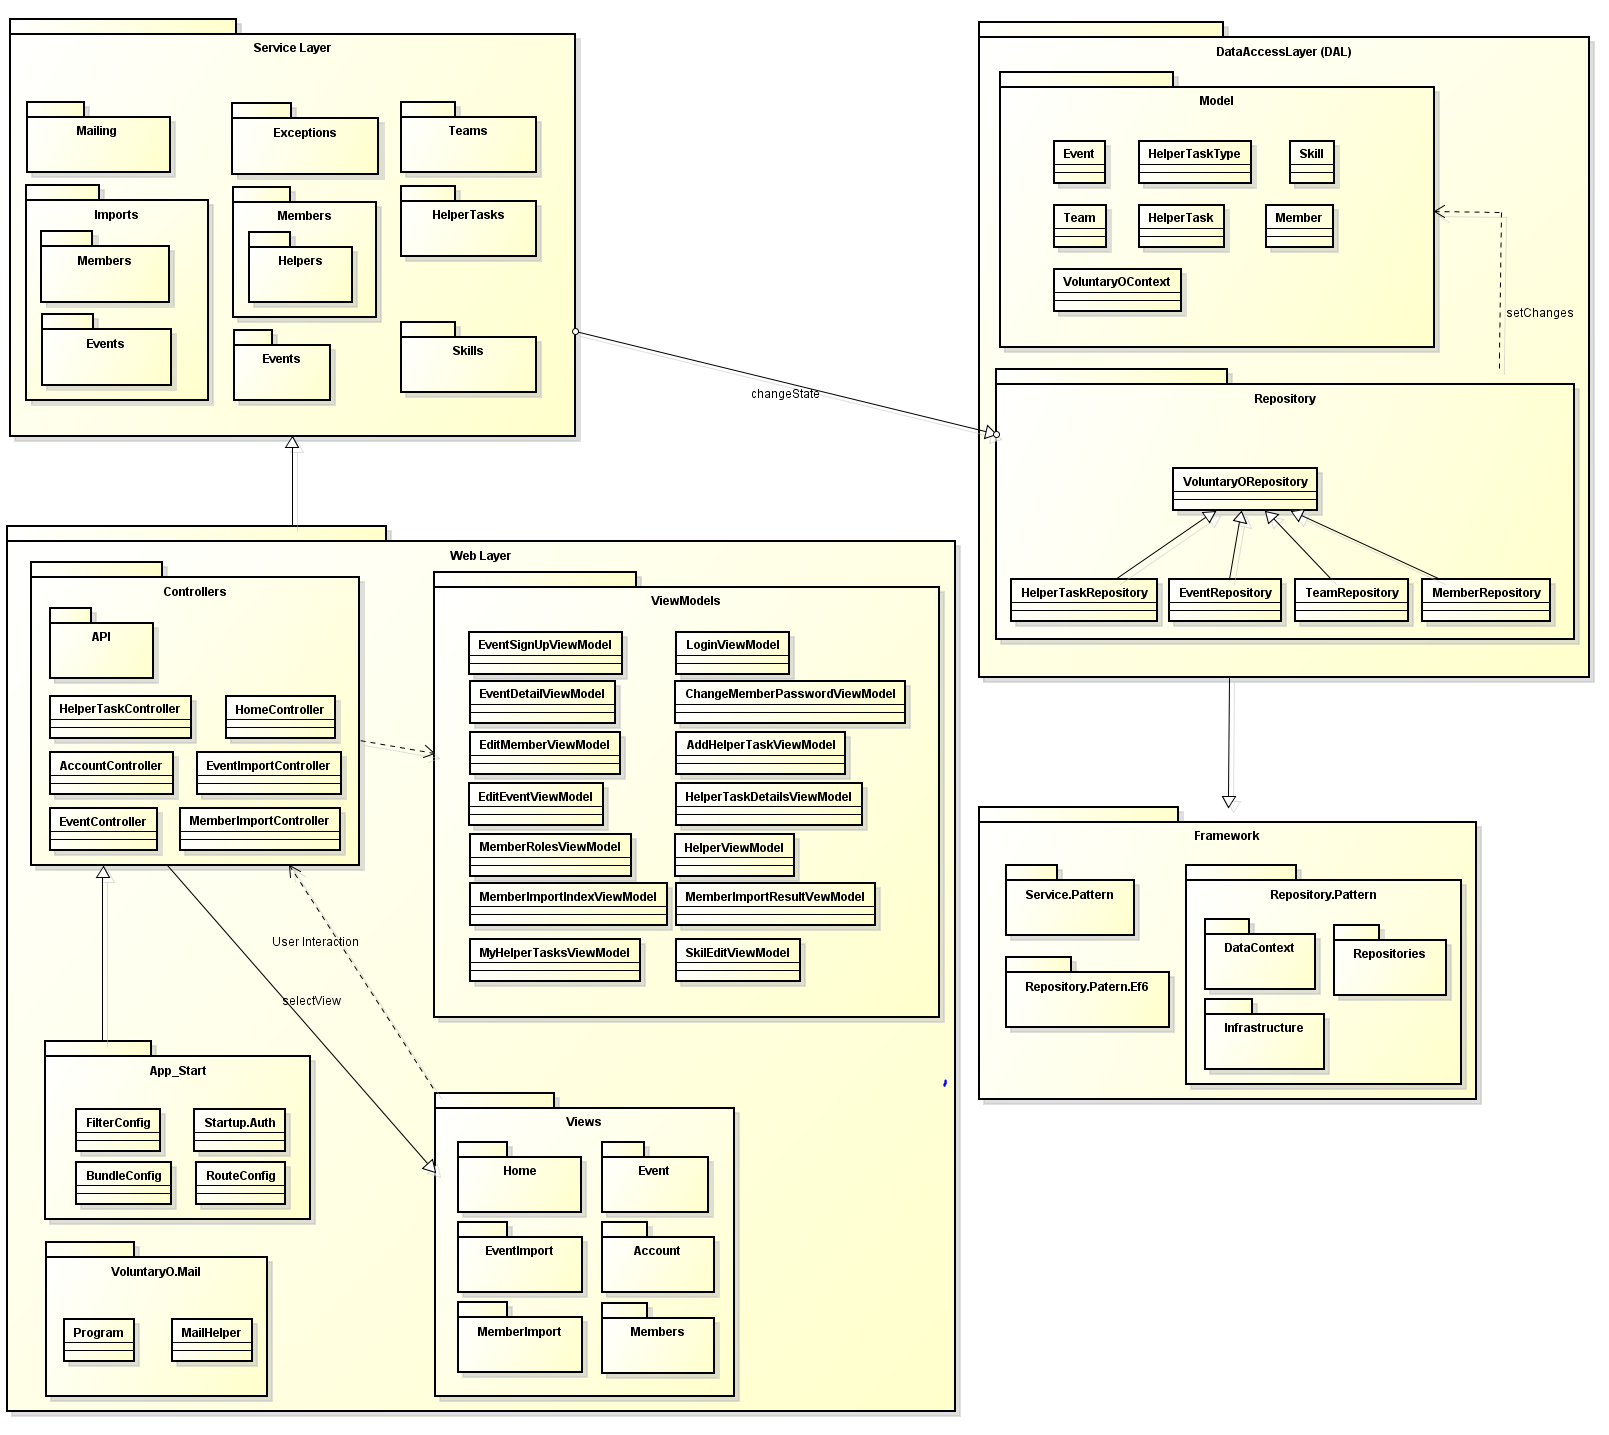
\includegraphics[width=\textwidth]{content/architekturdokumentation/images/LogischeArchitektur.png}
  		\vspace{-20pt}
    	\caption{Logische Architektur}
	\end{figure}

\newpage
\section{VoluntaryO.Dal (Data Access Layer)}
    \begin{figure}[h]
  		\vspace{-5pt}
    	\centering
    	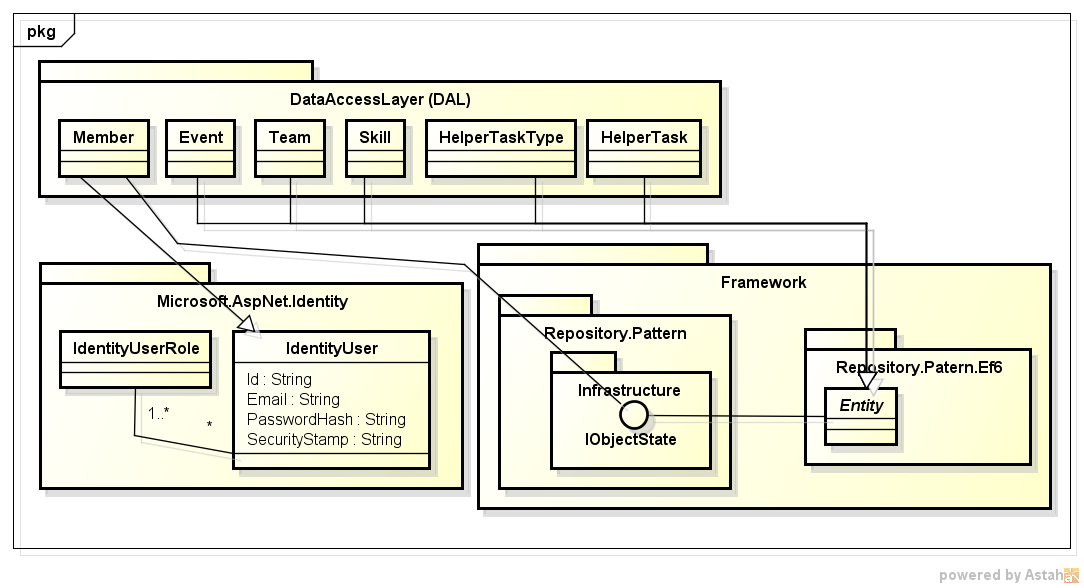
\includegraphics[width=0.7\textwidth]{content/architekturdokumentation/images/VoluntaryO_Dal_Overview.png}
  		\vspace{-20pt}
    	\caption{Klassen in VoluntaryO.Dal}
	\end{figure}
	Jede Model-Klasse implementiert die Schnittstelle \textit{IObjectState}, resp. leitet von der abstrakten Klasse \textit{Entity} ab. Die Verwendung von ASP.NET Identity ist im Kapitel VoluntaryO.Web näher beschrieben.
	
	\subsection{Vergleich für Objekte}
		Einzig für die Member-Klasse wurde die Vergleichsmethode (Equals) überschrieben. Folgende Attribute der Klasse sind relevant:
		\\\begin{itemize}
			\item \textit{UserName}
			\item \textit{Firstname}
			\item \textit{Lastname}
			\item \textit{Birthdate}
		\end{itemize}
		Der Vergleich wurde nur für die Mitgliedsimport-Funktion überschrieben. Für die übrigen Model-Klassen wird die standard Vergleichsmethode beibehalten (Vergleich der Referenz bei Referenztypen).

	\subsection{Repository / Unit of Work Pattern}
		Durch die Verwendung des \href{https://genericunitofworkandrepositories.codeplex.com/}{\textit{Generic Unit of Work \& Repositories Framework}} (in "'Framework"' abgelegt) ergeben sich folgende Vorteile:
		\\\begin{itemize}	
			\item Austauschbarkeit ORM
			\item Testbarkeit
			\item Jeder Request hat eigene Unit of Work (siehe später Dependecy Injection)
			\item Reduktion der Datenbankabfragen, da nur noch über Unit of Work commited wird
			\item Generische Abfragen von Entitäten
		\end{itemize}
		Folgende Konventionen ergeben sich aus für das Projekt:
		\\\begin{itemize}
			\item Jede Entität implementiert \textit{IObjectState}
			\item Repository kann über \textit{partial Classes} erweitern werden
			\item Oder Repository Klassen implementieren \textit{IRepository} und erben von \textit{Repository}
		\end{itemize}

	\subsubsection{Konventionen für eigene Repository Erweiterungen}
		\begin{itemize}
			\item Objekt(-e) abrufen/suchen \textit{Find*}
			\item Objekt(-e) einfügen \textit{Insert*}
			\item Objekt ändern \textit{Update*}
			\item Objekt hinzufügen \textit{Delete*}
			\item Zuweisung zweier Objekte hinzufügen \textit{Assign*}
			\item Zuweisung zweier Objekte entfernen \textit{Unassign*}
		\end{itemize}

	\subsection{Unit Tests mit Effort}
		\href{https://effort.codeplex.com/}{\textit{Effort}} ist ein ADO.Net Provider und erstellt jeweils eine In-Memory Datenbank für das EF. Die temporäre Datenbank ermöglicht uns ein Testen des Codes, ohne Datenbankzugriffe zu mocken.
		\begin{lstlisting}[language=CSharp, caption=Verwendung Effort für Unit Tests in EffortTest.cs, label=lst:effortunittest, firstnumber=1]
			DbConnection Connection = DbConnectionFactory.CreateTransient();
			VoluntaryoContext VoluntaryoContext = new VoluntaryoContext(_Connection);
	    \end{lstlisting}
	    Den einzelnen Unit Tests steht so eine saubere und testbare Datenbank zur Verfügung. Jeder UnitTest erbt von der Abstrakten Klasse \textit{EffortTest}.

	\subsection{Relationales Modell}
	    \begin{figure}[h]
	  		\vspace{-5pt}
	    	\centering
	    	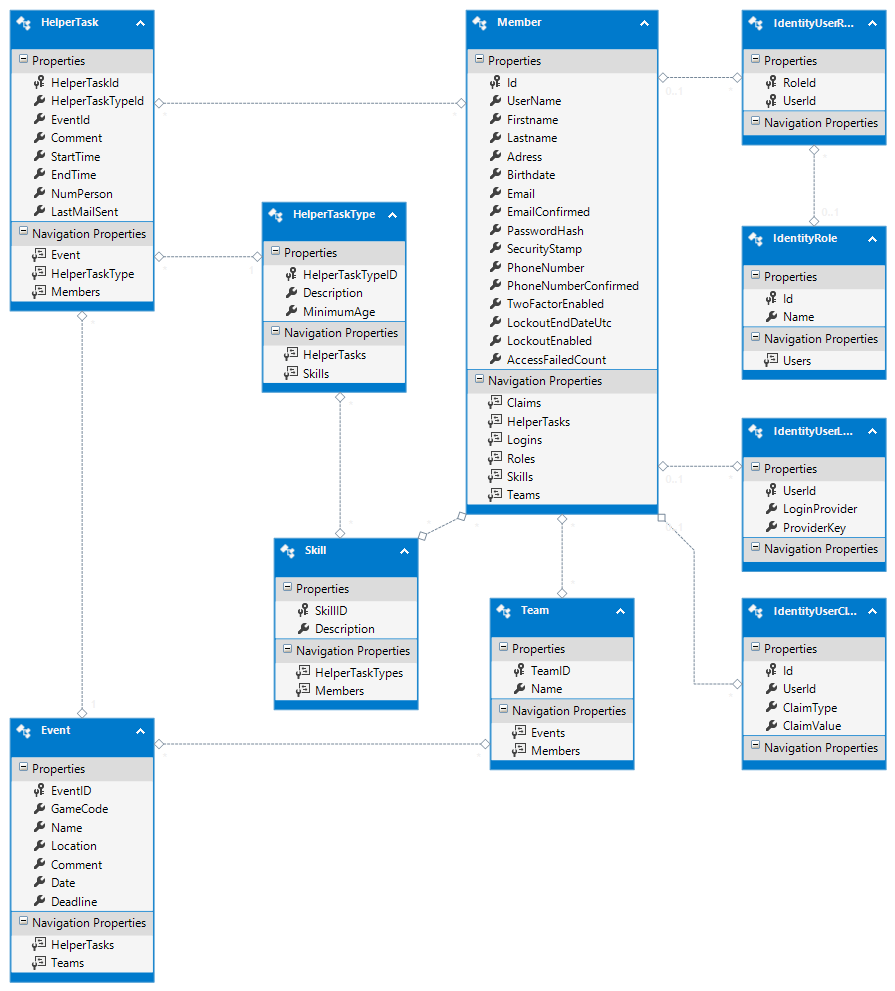
\includegraphics[width=0.7\textwidth]{content/architekturdokumentation/images/edmx.png}
	  		\vspace{-20pt}
	    	\caption{Relationales Modell für VoluntaryO.Dal}
		\end{figure}
		\subsubsection{Mapping}
			Das Mapping wird mit dem \textit{modelBuilder} des EF gesteuert. Bspw.
			\begin{lstlisting}[language=CSharp, caption=Mapping in VoluntaryoContext.cs, label=lst:mappingcontextcs, firstnumber=1]
	// TeamEventMapping
	modelBuilder.Entity<Team>()
	    .HasMany(t => t.Events)
	    .WithMany(e => e.Teams)
	    .Map(mc =>
	    {
	        mc.MapLeftKey("TeamID");
	        mc.MapRightKey("EventID");
	        mc.ToTable("TeamEventMappings");
	    });
		    \end{lstlisting}

\newpage
\section{VoluntaryO.Service}
	Dieses Subprojekt dient als Abstraktionsschicht zwischen den Packages aus dem DAL und deren Verwendung im Web Layer und enthält die eigentliche Business-Logik. Dadurch wird die Logik in den Actions der Controller reduziert und eine höhere Kohäsion erreicht. Die Aufteilung  von Namespaces und Ordner wurde aufgrund der Zugehörigkeit zu den Entitätsklassen im Domainmodell gewählt. Aufgabenspezifische Service-Komponenten wurden ebenfalls in der obersten Hierarchiestufe des Service-Projekts in einem separaten Ordner untergebracht.
	
	\begin{figure}[H]
	    	\centering
	    	 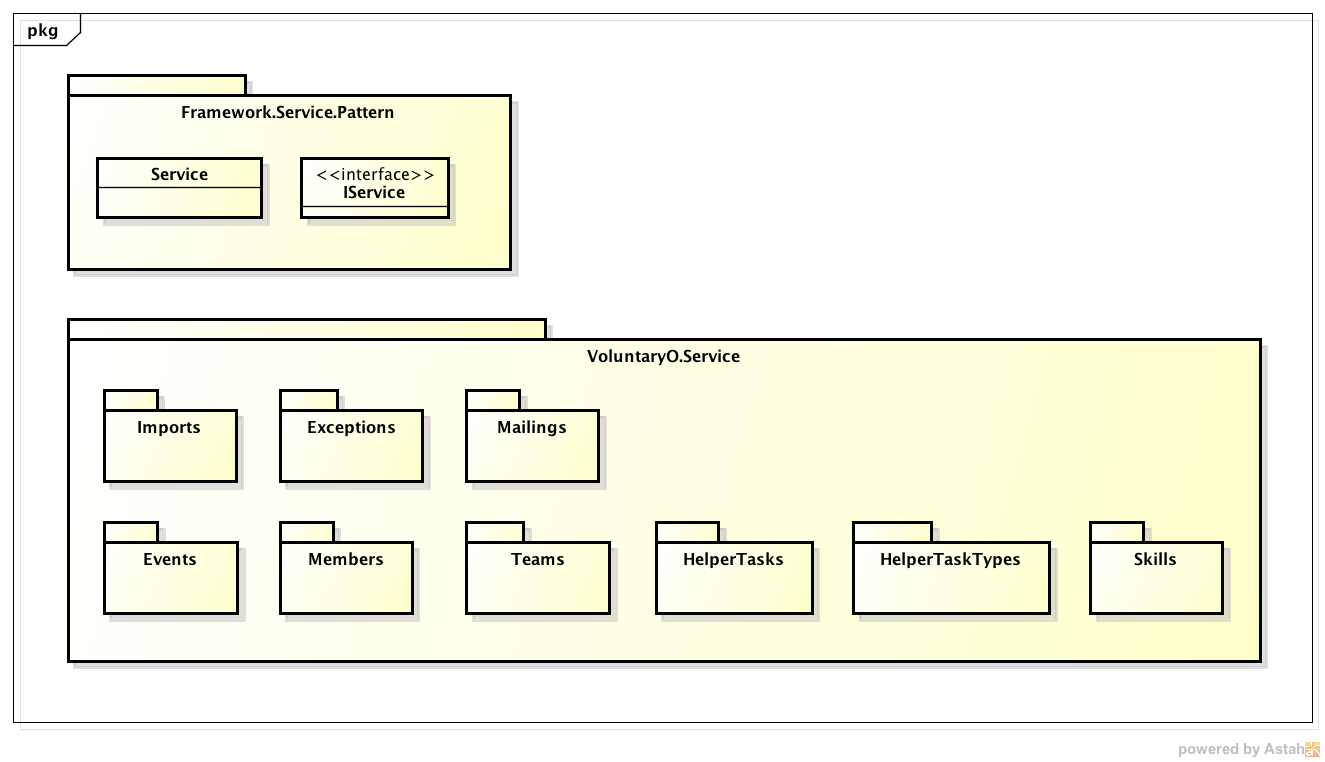
\includegraphics[width=0.9\textwidth]{content/architekturdokumentation/images/Service_Overview.png}
	  		\vspace{-25pt}
			\caption{Packageübersicht des Service-Layers und Service Pattern}
	\end{figure}
	
	\subsection{Verwendung der Service-Klassen}
	Für jedes Repository existiert eine zugehörige Service-Klasse, welche das \textit{IService} Interface implementiert. Dadurch wird die Kopplung zwischen Respositories und Controllern reduziert und eine einheitliche Schnittstelle zur Business-Logik geschaffen:
	
	\begin{figure}[H]
	    	\centering
	    	 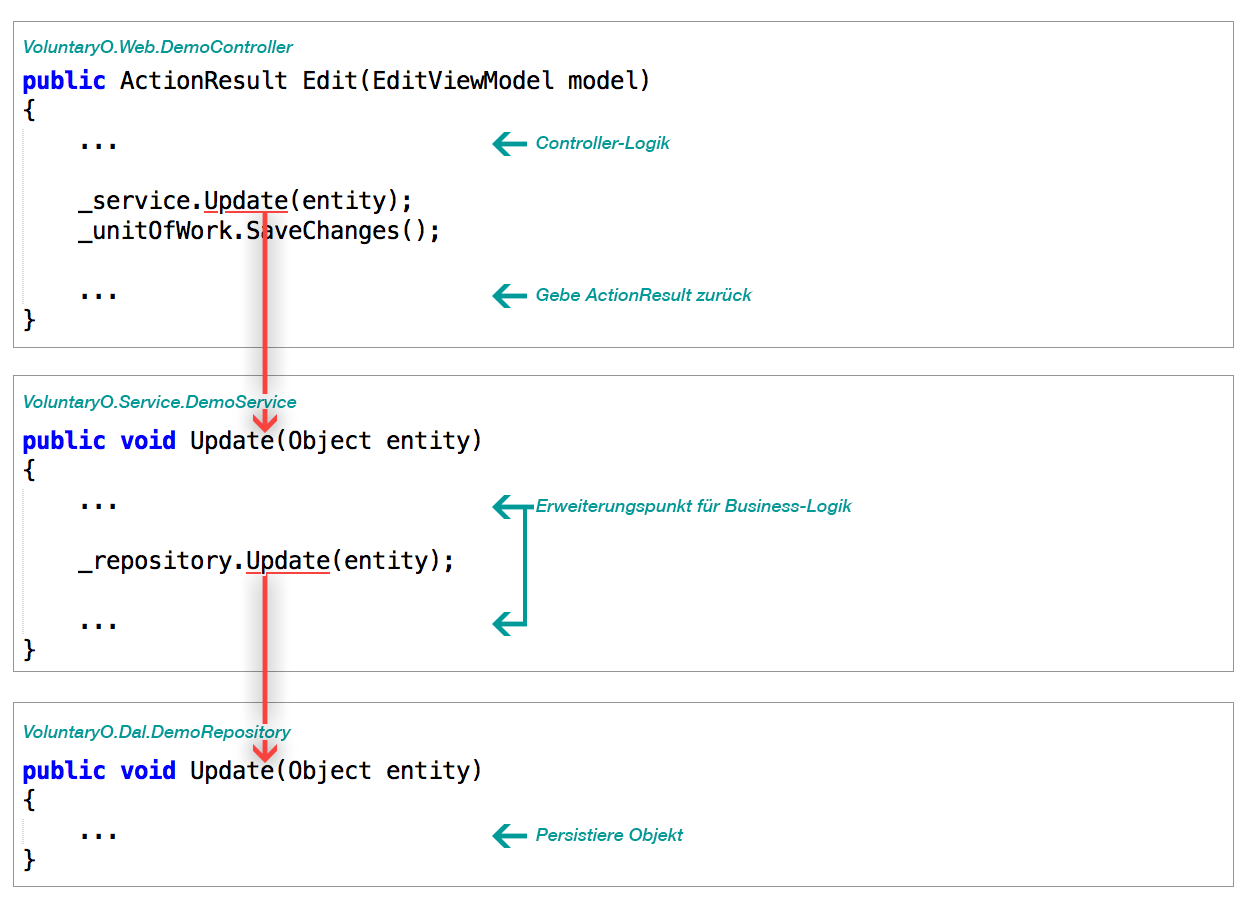
\includegraphics[width=0.9\textwidth]{content/architekturdokumentation/images/Service_Framework_Code.png}
	  		\vspace{-15pt}
			\caption{Aufrufhierarchie über Layers anhand eines Beispiels}
	\end{figure}
	
	\subsection{Aufbau der Service-Klassen}
	Die Vererbungshierarchie aller Service-Klassen (Ausnahme: MailingService) folgt immer dem selben Schema. Dadurch kann ein einheitliches Design verwendet werden und es ist klar, wo Erweiterungen integriert werden können.
	
	\begin{figure}[H]
	    	\centering
	    	 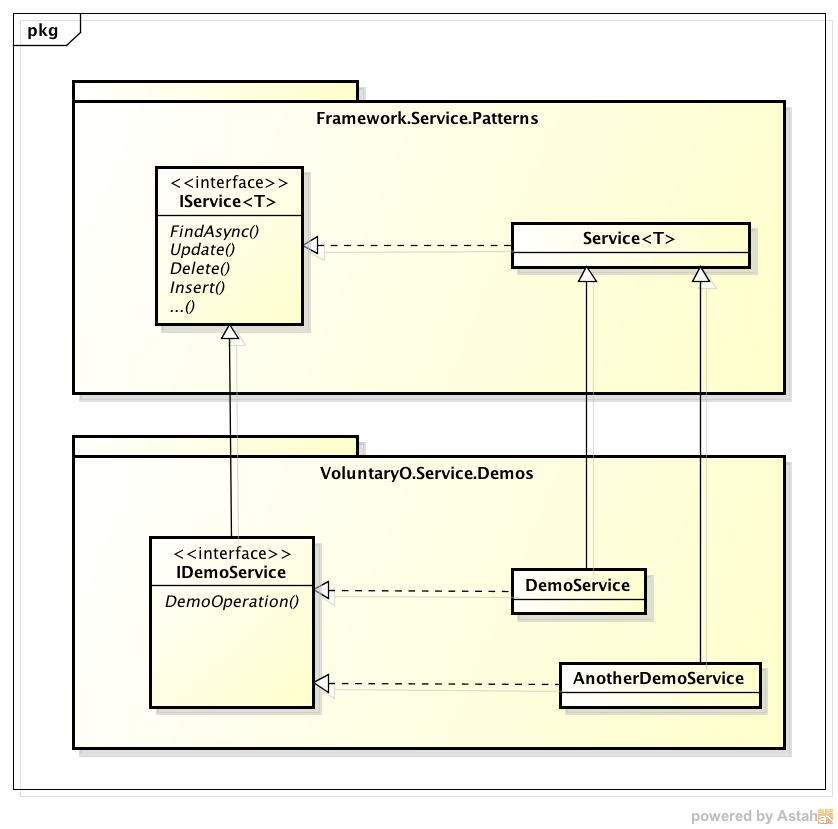
\includegraphics[width=0.9\textwidth]{content/architekturdokumentation/images/Service_Class_Hierarchy.png}
	  		\vspace{-15pt}
			\caption{Referenz-Hierarchie für Service-Klassen}
	\end{figure}
	
	Pro Repository wird ein Interface definiert (\textit{IDemoService}), welches alle spezifischen Methoden vorgibt. Jede Implementierung dieser Schnittstelle (\textit{DemoService, AnotherDemoService}) erbt zusätzlich von \textit{Service}. Der Dependency Injection Container (Unity) ist verantwortlich für die Instanziierung der richtigen Implementierung.
	
	
	\subsection{Service-Klassen im Überblick}
	

	
	\subsubsection{MemberService}
	
	Die MemberService-Klasse funktioniert als Schnittstelle zum MemberRepository. Speziell hervorzuheben ist die \textit{ImportMember}-Methode. Sie erlaubt es, freistehende Member-Objekte (externe Members), die nicht aus dem Repository stammen, kollisionsfrei zu integrieren.
	
	\begin{table}[H]
        \tablestyle
        \tablealtcolored
        \begin{tabularx}{\textwidth}{X X}
        \tableheadcolor
            \tablehead Methode & 
            \tablehead Beschreibung \\  
        \tablebody
            bool CheckIfMemberExists(Member member) & 
            Überprüft, ob ein Mitglied mit selbem Vornamen, Nachnamen und Geburtsdatum existiert. Falls nicht, wird davon ausgegangen, dass diese Person noch nicht im System vorhanden ist.  \tabularnewline
            
            bool CheckIfMemberWasModified(Member member) &
            Überprüft, ob das Mitglied existiert und Kontaktdaten oder Teamzugehörigkeit gewechselt haben. \tabularnewline
            
			Boolean ImportMember(Member member) &
			Versucht externe Members im System zu speichern. Dabei wird unterschieden, ob es sich um ein neues Mitglied, ein bestehendes mit abweichenden Angaben oder ein bestehendes, unverändertets Mitglied handelt. \tabularnewline      
			
			bool ImportMember(Member member, bool overwriteIfModified) &
			Importiert externe Members und überschreibt bestehende Member-Objekte, falls das \textit{overwriteIfModified}-Flag gesetzt wurde. \tabularnewline
            
			void UpdateMember(Member member)  &
			Aktualisiert Kontaktdaten und Teamzugehörigkeit eines Mitglieds. \tabularnewline
			
			void AssignMemberAndTeamWithInsert(Member member, string teamName) &
			Weist dem Mitglied ein echtes Team-Objekt aus dem Repository zu oder erstellt ein solches anhand des übergebenen Strings, falls es noch nicht existiert. \tabularnewline
			
			ICollection<Member> UnmodifiedRecords() &
			Externe Members, die beim Importieren übersprungen wurden, weil sie nicht verändert wurden. \tabularnewline
			
			ICollection<Member> ModifiedRecords() &
			Externe Members, die verändert und deshalb nicht abgespeichert wurden. \tabularnewline
			
			ICollection<Member> NewRecords() &
			Externe Members, die zuvor noch nicht im System vorhanden waren und abgespeichert wurden. \tabularnewline
			
				
			         
        \tableend
        
        \end{tabularx} 
    \end{table}
	
	
	\subsection{EventService}
		Der EventService verbindet den EventController mit dem Event- und HelperTaskRepository. Die Logik zum Verwalten der Relationen zwischen Helfereinsätzen, Events Mannschaften wurde hier implementiert.
		
		\begin{table}[H]
        \tablestyle
        \tablealtcolored
        \begin{tabularx}{\textwidth}{X X}
        \tableheadcolor
            \tablehead Methode & 
            \tablehead Beschreibung \\  
        \tablebody
            void AssignEventAndTeam(int eventId, int teamId) & 
            Fragt Event und Team anhand von Id's aus den Repositories ab und stellt die Relation her.  \tabularnewline
            
            void UnassignEventAndTeam(int eventId, int teamId) & 
            Fragt Event und Team anhand von Id's aus den Repositories ab und hebt die Relation auf.  \tabularnewline
            
           void InsertHelperTask(HelperTask task, int taskType, int eventId) &
           Selektiert Event- und HelperTask-Objekte, um dem Event einen Helfereinsatz zuzuordnen. \tabularnewline
           
           void DeleteHelperTask(int helperTaskId) &
           Löscht den Helfereinsatz anhand der Id. Das Event wird dazu nicht benötigt. \tabularnewline
           
           void UnassignEventAndAllTeams(Event e) &
           Entfernt alle Teams eines Events. \tabularnewline
           
           void	UnassignEventAndAllHelperTasks(Event e) &
           Entfernt alle Helfereinsätze eines Events. \tabularnewline
           
           void AssignEventAndTeam(Event e, Team team) &
           Ordnet dem Event ein weiteres zuständiges Team zu. \tabularnewline
           
           void AssignEventAndHelperTask(Event e, int helperTaskId) &
           Ordnet dem Event einen weiteren Helfereinsatz zu. \tabularnewline
           
                     
           
           bool Contains(Event e) &
           Überprüft, ob ein Event bereits im Repository existiert. \tabularnewline

			
            IEnumerable<Event> FindEventsBySearchStringWithSortOrder(string searchString, string sortOrder) &
            Findet Events, die im Namen, Datum, Ort oder Team mit dem übergebenen Such-String übereinstimmen. Zusätzlich kann die Sortierung gesteuert werden. Erlaubte Werte sind ``Location'',  ``location\_desc'', ``Deadline'', ``deadline\_desc'', ``Name'', ``name\_desc'' und ``date\_desc''. Die Standardsortierung wird anhand von ``Date'' vorgenommen. \tabularnewline 
				
			         
        \tableend
        
        \end{tabularx} 
    \end{table}
	
	\subsection{TeamService}
		Bietet Zugriff auf die Methoden des TeamRepository und stellt Erweiterungspunkt für komplexere Logik dar. Diese Klasse wird im \textit{EventController} verwendet.
		
		\begin{table}[H]
        \tablestyle
        \tablealtcolored
        \begin{tabularx}{\textwidth}{X X}
        \tableheadcolor
            \tablehead Methode & 
            \tablehead Beschreibung \\  
        \tablebody
            IEnumerable<Team> GetAllTeams() & 
            Selektiert alle Teams aus dem Repository.  \tabularnewline
            
            Team GetTeamById(int id) &
            Selektiert Team aus Repository anhand der Id. \tabularnewline
	
			         
        \tableend
        
        \end{tabularx} 
    \end{table}
		
	
	\subsection{SkillService}
		Bietet Zugriff auf die Methoden des SkillRepository und stellt Erweiterungspunkt für komplexere Logik dar.
		
		\begin{table}[H]
        \tablestyle
        \tablealtcolored
        \begin{tabularx}{\textwidth}{X X}
        \tableheadcolor
            \tablehead Methode & 
            \tablehead Beschreibung \\  
        \tablebody
            public IEnumerable<Skill> GetAllSkills() & 
            Selektiert alle Skills aus dem Repository.  \tabularnewline
	
			         
        \tableend
        
        \end{tabularx} 
    \end{table}
	
	\subsection{HelperTaskService}
		Die HelferTaskService-Klasse wird von mehreren Controllern verwendet. Sie enthält wichtige Business-Logik zum An- und Abmelden für einen Helfereinsatz und prüft dazu folgende Bedingungen:
		\\\begin{itemize}
			\item Helfereinsatz ist noch nicht mit ausreichend vielen Mitgliedern belegt
			\item Mitglied hat sich noch nicht für diesen Helfereinsatz angemeldet
			\item Keine Zeitüberschneidung mit anderen Helfereinsätzen vorhanden
			\item Fähigkeiten für den Einsatz sind gegeben
		\end{itemize}
		
		\begin{table}[H]
        \tablestyle
        \tablealtcolored
        \begin{tabularx}{\textwidth}{X X}
        \tableheadcolor
            \tablehead Methode & 
            \tablehead Beschreibung \\  
        \tablebody
           void SubmitForTask(Member member, HelperTask task) & 
           Versucht, das Mitglied für einen Helfereinsatz zu registrieren. Dazu müssen alle oben genannten Bedinungen erfüllt sein. \tabularnewline
           
           void RemoveFromTask(Member member, HelperTask task) &
           Meldet das Mitglied wieder vom Helfereinsatz ab. \tabularnewline
           
           void UnassignAllMembers(HelperTask helperTask) &
           Meldet alle Mitglieder eines Helfereinsatzes ab. \tabularnewline
           
           
	
		\tableend
        
        \end{tabularx} 
    \end{table}
	
	\subsection{Imports}
		Für das Importieren von Mitgliedern und Events wird jeweils eine eigene Serviceklasse verwendet. Die abstrakte Klasse \textit{Importer} dient dazu als Basis und schreibt die Methode \textit{executeImport} vor.
		
	    \begin{figure}[h]
	  		\vspace{-5pt}
	    	\centering
	    	 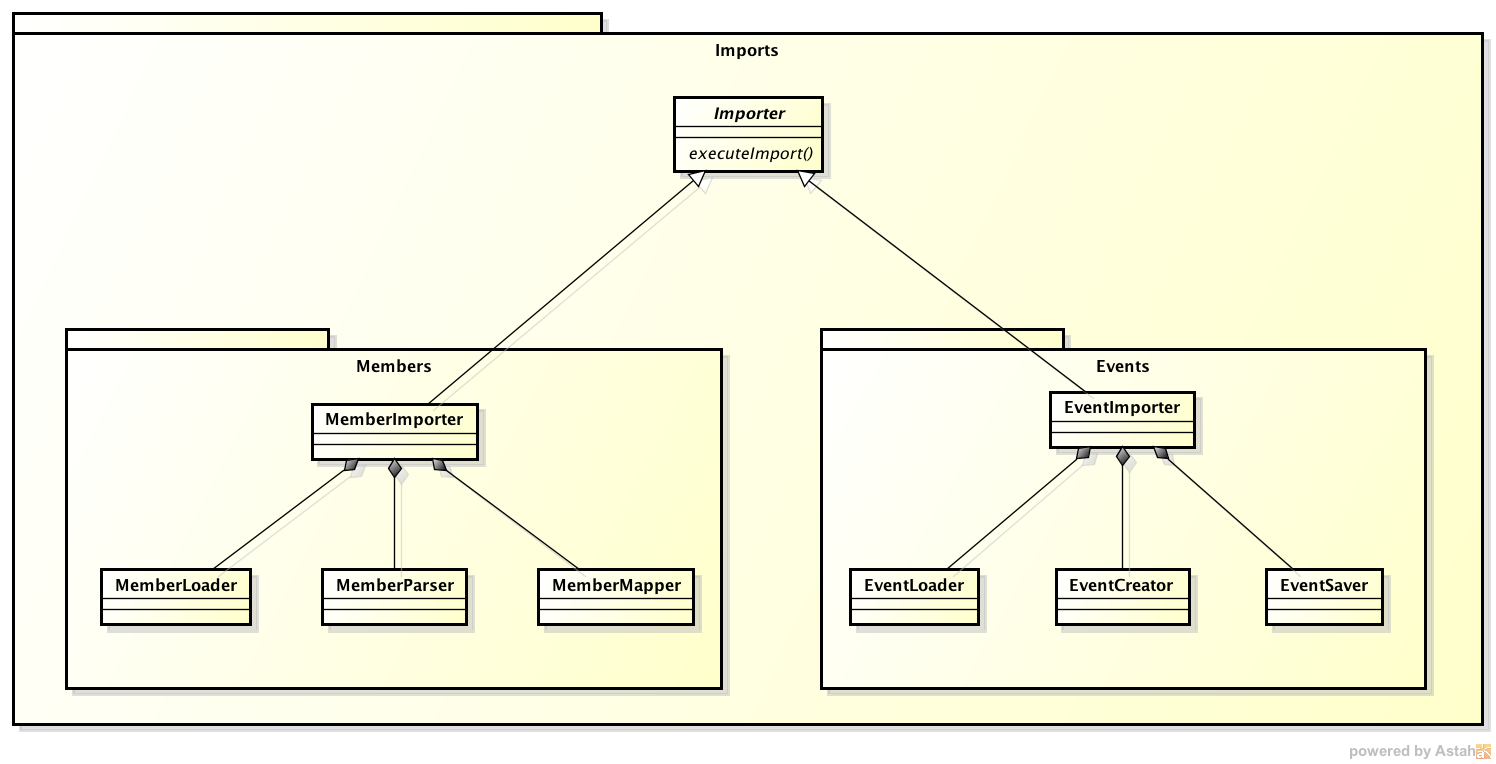
\includegraphics[width=0.9\textwidth]{content/architekturdokumentation/images/ImportPackageDesign.png}
	  		\vspace{-25pt}
			\caption{Importer-Klassen und deren direkte Collaborators}
		\end{figure}
		
		\subsubsection{MemberImporter}
			Der MemberImporter implementiert die Methode \textit{executeImport}, welche das importieren von Mitgliedern startet. Um eine höhere Kohäsion und niedrige Kopplung zu erreichen, wurden die Teilaufgaben ausgelagert:
			\\\begin{itemize}	
				\item MemberLoader - benutzt die webling.ch Schnittstelle und lädt das CSV
				\item MemberParser - liest den CSV-String und speichert die Werte in eine Liste von Hashtables
				\item MemberMapper - gibt Member-Objekte an MemberService zum Speichern weiter\\
			\end{itemize}



		\subsubsection{EventImporter}
			Der EventImporter implementiert ebenfalls die von der abstrakten Basisklasse \textit{Importer} vorgebenen Methode zum Auslösen der Import-Routine. Auch hier wurde die Arbeit in drei Teilaufgaben gegliedert:
			\\\begin{itemize}	
				\item EventLoader - lädt die Daten vom Swiss Unihockey REST Service
				\item EventCreator - liefert Liste mit Event-Objekten
				\item EventSaver - Speichet die Events in der Datenbank ab\\
			\end{itemize}
	
			\noindent
			Da Events in der Regel nur einmal pro Saison importiert werden, müssen diese nicht auf Modifikationen überprüft werden.
	
	\subsection{MailingService}
		Um das Versenden von E-Mails zu vereinfachen, kapselt diese Klasse die Vorbereitung und Konfiguration eines \textit{SmtpClient} und einer \textit{MailMessage}. Dabei werden SMTP-Host und -Port, sowie die Credentials aus dem \textit{ConfigurationManager} gelesen.  

		\begin{lstlisting}[language=CSharp, caption=Verwendung des MailingService, label=lst:mailingservice, firstnumber=1]
	var mail = new MailingService();
	mail.SendMail("nle@hsr.ch", "nle@hsr.ch", "Test Subject", "Test Message");
	    \end{lstlisting}
    



\section{VoluntaryO.Web}
	Die komplette Implementierung des Frontends befindet sich im Projekt Voluntary.Web. Folgend wird beschrieben, wie VoluntaryO.Web aufgebaut ist und welche Konzepte verwendet wurden um die Darstellung des Frontends zu erreichen.

	\subsection{Projektaufbau}
		VoluntaryO.Web ist ein Projekt innerhalb der Solution. Der Projektaufbau wird in der Reihenfolge der Ordner beschrieben.

		\begin{figure}[H]
	    	\centering
	    	 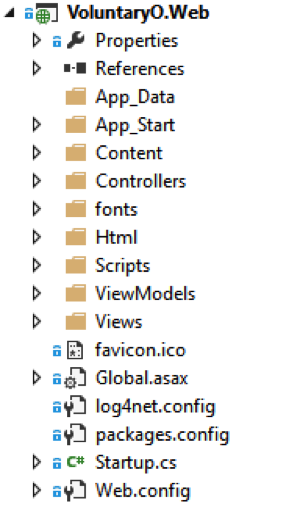
\includegraphics[width=0.3\textwidth]{content/architekturdokumentation/images/web-1-Projektaufbau.png}
	  		\vspace{-10pt}
			\caption{Projektaufbau VoluntaryO.Web}
		\end{figure}

		\subsubsection{References}
			Das Projekt hat Referenzen auf VoluntaryO.Dal und VoluntarO.Service um auf die Datenpersistenz zugreifen zu können. Andere Referenzen ergeben sich automatisch durch den Einsatz von Entity Framework, und ASP.NET MVC.
		
		\subsubsection{AppStart}
			Hier werden wichtige Konfigurationen für ASP.NET vorgenommen. Besonders herauszuheben ist hier BundleConfig.cs. Unser Projekt bietet sechs verschiedene Bundles an. Jedes Bundle besteht aus mehreren CSS oder JS Files, die innerhalb eines Bundles in einem minimierten File an den Client ausgeliefert werden (Nur in Realese-Deploy). Dies bietet den Vorteil, dass während der Entwicklung der JS-Code gedebuggt werden kann und später eine möglichst hohe Effizien erreichbar ist. Ausserdem bietet Bundle-Config eine zentrale Managementlösung für JS- und CSS-Files.
			Im AppStart wird ausserdem die Konfiguration der Dependency Injection vorgenommen.
			Die Idee hinter Dependency Injection und allgemein Inversion-of-Control, ist die Anwendung des sogenannten Hollywood Prinzips: \"Don’t call us, we call you!\". 
			\\Als Dependency Injection Container wird \href{http://unity.codeplex.com/}{Unity} verwendet. Der Controller gibt in seinem Konstruktor an, welche Interfaces benötigt werden. \textit{Unity} wird diese Abhängigkeiten dann zur Laufzeit zur Verfügung stellen.
			\begin{lstlisting}[language=CSharp, caption=UnityConfig.cs, label=lst:unityconfig, firstnumber=1]
			container.RegisterType<IDataContextAsync, VoluntaryoContext>(new PerRequestLifetimeManager(), new InjectionConstructor())
		    .RegisterType<IUnitOfWork, UnitOfWork>(new PerRequestLifetimeManager())
		    .RegisterType<IUnitOfWorkAsync, UnitOfWork>(new PerRequestLifetimeManager())
		    .RegisterType<IEventRepository, EventRepository>()
		    .RegisterType<IHelperTaskRepository, HelperTaskRepository>()
		    .RegisterType<IRepository<HelperTaskType>, Repository<HelperTaskType>>()
		    .RegisterType<IMemberRepository, MemberRepository>()
		    .RegisterType<ITeamRepository, TeamRepository>()
		    .RegisterType<IRepositoryAsync<Skill>, Repository<Skill>>()
		    .RegisterType<IEventService, EventService>()
		    .RegisterType<IHelperTaskService, HelperTaskService>()
		    .RegisterType<ISkillService, SkillService>()
		    .RegisterType<IMemberService, MemberService>()
		    .RegisterType<ITeamService, TeamService>();
		    \end{lstlisting}
		    Der \textit{PerRequestLifetimeManager} hält die Instanz für den gesamten HTTP-Request. Somit erhält jeder Request ein eigener \textit{Context} und eine eigene \textit{Unit of Work}.
		    Zuletzt wird in AppStart noch die Konfiguration des Routings zum Web-API vorgenommen.

		\subsubsection{Content}
			Der Ordner Content enthält alle Bilder und CSS-Files, die für das Projekt benötigt werden. Diese sind unter anderem Bootstrap, Chosen und spezifische CSS –Files für VoluntaryO.

		\subsubsection{Controllers}
			Die Controller sind ein essentieller Teil des MVC-Patterns (Model-View-Controller), das wir durch ASP.NET verwenden.

			\begin{figure}[H]
		    	\centering
		    	 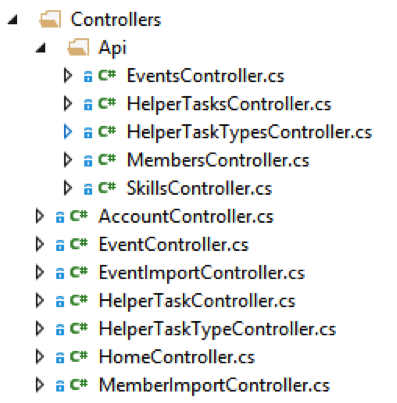
\includegraphics[width=0.5\textwidth]{content/architekturdokumentation/images/web-2-Controllers.png}
		  		\vspace{-5pt}
				\caption{Controllers}
			\end{figure}

			Sobald im Client eine URL mit folgendem Schema aufgerufen wird:
			/{controller}/{methode}
			Wird innerhalb des Controllers mit dem jeweiligen Name die jeweilige Methode aufgerufen. Für jede Methode innerhalb eines Controllers gibt es eine gleichnamige View im Ordner Views.
			In jeder Methode innerhalb des Controllers wird festgelegt, welche Rollen darauf zugreifen können.

			\begin{lstlisting}[language=CSharp, caption=EventController.cs, label=lst:Details firstnumber=1]
			// GET: /Event/Details/5
	        [Authorize(Roles = "Admin,Planer,Member")]
	        public ActionResult Details(int? id)
	        {
	            if (id == null)
	            {
	                return new HttpStatusCodeResult(HttpStatusCode.BadRequest);
	            }
	            var e = _eventService.Find((int) id);
	            if (e == null)
	            {
	                return HttpNotFound();
	            }
	            var model = new EventDetailViewModel(e, _teamService.GetAllTeams().ToList());
	            return View(model);
	        }
			\end{lstlisting}

			Speziell ist hier noch der Folder API. Er wird von verschiedenen Views benutzt um von der Client-Side über AJAX asynchrone Requests auf die Applikation auszuführen. Die Methoden sind hier nach den verschiedenen HTTP-Request-Codes benannt (GET, POST, DELETE usw.)

		\subsubsection{Scripts}
			Innerhalb des Folders Scripts sind alle JS-Files abgelegt. Grundsätzlich sind diese in Bootstrap, Chosen, FullCalender, JQuery und spezifische VoluntaryO-Scripts zu unterteilen. Die Scripts werden durch die zuvor beschriebenen Bundles in der View angezeigt.

		\subsubsection{View Models}

			\begin{figure}[H]
		    	\centering
		    	 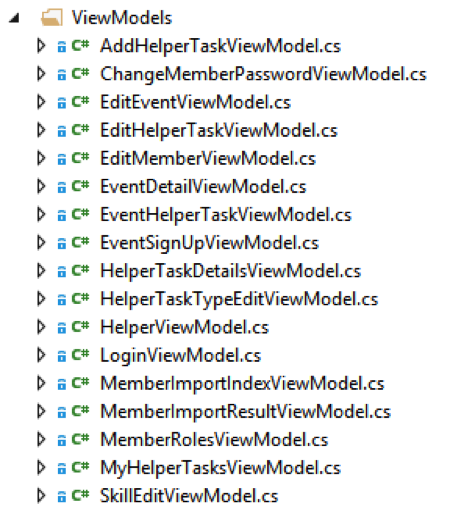
\includegraphics[width=0.5\textwidth]{content/architekturdokumentation/images/web-3-ViewModels.png}
				\caption{ViewModels}
			\end{figure}

			Um die Websiten dynamisch darzustellen nutzen wir die ASP.NET Razor View Engine. Eine Razor-View ist immer mit einer Methode des Controllers verbunden. Das bedeutet auch, dass der Return-Wert der Methode sämtliche Daten mitliefern muss, die später in der View gebraucht werden. Da in einer View häufig mehr als nur ein standard Objekt aus dem Model gebraucht wird, haben viele Views ein Extra Viewmodel. Das bedeutet es wird extra eine Instanz eines speziell auf die View zugeschnittenen Objekt erstellt. Dieses View-Model enthält alle Referenzen auf andere Objekte, die innerhalb der View gebraucht werden. Durch den Einsatz des View-Model haben wir den Vorteil, dass pro View genau definiert ist, welche Daten wir brauchen. Der Zugriff auf das View-Model kann einfach getestet werden. Der Einsatz eines View-Models bietet aber auch einige Nachteile, beispielsweise werden manche Methoden redundant implementiert. Da wir die Implementation der Methoden aber sowieso auf die Service-Schicht abstrahiert haben, birgt dies für uns kein Problem. Da wir nicht durch das Model pro View eingeschränkt werden wollen bietet uns das View-Model den besten Dienst.

		\subsubsection{Views}

			\begin{figure}[H]
		    	\centering
		    	 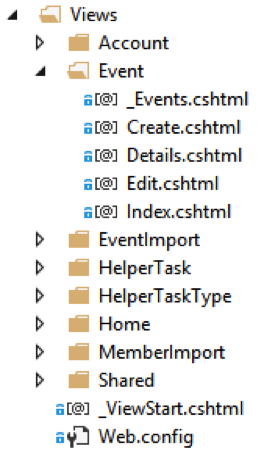
\includegraphics[width=0.3\textwidth]{content/architekturdokumentation/images/web-4-Views.png}
		  		\vspace{-10pt}
				\caption{Views}
			\end{figure}

			Alle Controller besitzen ein entsprechendes Pendant im Ordner Views. Hier sind alle .cshtml Files abgelegt, die vom Client angezeigt werden können.
			Detailliert sieht man das innerhalb des Ordners Event. Für die Events gibt es eine Ansicht in Listenstruktur (Index), eine Detail-Ansicht (Details) und eine Erstell und Editier-Funktion (Create \& Edit). Alle Files die mit einem Underscore beginnen (\_Events) sind Partial-Views die innerhalb anderer Views wiederverwendet werden können.

			In den Views ist auch der Javascript-Code zu finden, welcher die AJAX-Befehle ausführt. Ein Beispiel:

			\begin{lstlisting}[language=javascript, caption=text/javascript, label=lst:AJAX Example firstnumber=1]
			$(document).ready(function() {
	            $("#team-selection").chosen({
	                allow_single_deselect: true
	            });

	            $(".remove-helperTask").confirmation({
	                onConfirm: function(e, element) {
	                    console.log($(element));
	                    e.preventDefault();
	                    $.ajax({
	                        type: 'DELETE',
	                        url: '/api/helperTasks/' + $("#helperTaskId").val(),
	                        success: function(data) {
	                            getHelperTasks($('#calendar'));
	                            $("#taskdetailform")[0].reset();
	                        },
	                        error: function(data) {
	                            console.log(data);
	                        }
	                    });
	                }
	            });
	        });
			\end{lstlisting}

	\subsection{Controllers}
		Folgend werden die vier wichtigsten Controller und der REST-API-Controller detailliert beschrieben
		\subsubsection{HomeController}
			
			\begin{table}[H]
		        \tablestyle
		        \tablealtcolored
		        \begin{tabularx}{\textwidth}{p{3cm} p{0.8cm} p{6cm} X p{1.2cm}}
		        \tableheadcolor
		            \tablehead Adresse & 
		            \tablehead HTTP &
		            \tablehead Beschreibung &
		            \tablehead Parameter &
		            \tablehead Rechte \\  
		        \tablebody
		        	/Home/Index &
		        	GET &
		        	Gibt alle offenen Helfereinsätze eines Members zurück &
		        	- &
		        	Admin, Planer, Member
		        	\tabularnewline
		        \tableend
		        \end{tabularx} 
		    \end{table}

		\subsubsection{EventController}

			\begin{table}[H]
		        \tablestyle
		        \tablealtcolored
		        \begin{tabularx}{\textwidth}{p{3cm} p{0.8cm} p{6cm} X p{1.2cm}}
		        \tableheadcolor
		            \tablehead Adresse & 
		            \tablehead HTTP &
		            \tablehead Beschreibung &
		            \tablehead Parameter &
		            \tablehead Rechte \\  
		        \tablebody
		        	/Event/Index &
		        	GET &
		        	Gibt alle Events zurück. Möglichkeit für Filterung und Sortierung. Falls über AJAX angefragt wird Partial View zurückggeben. &
		        	string sortOrder
					string searchString &
		        	Admin, Planer, Member
		        	\tabularnewline

		        	/Event/Details/{id} &
		        	GET &
		        	Gibt details eines Events als EventDetailViewModel zurück &
		        	int? Id &
		        	Admin, Planer, Member
		        	\tabularnewline

		        	/Event/DeleteTeam &
		        	GET &
		        	Entfernt Teamzuweisung aus einem spezifischen Event &
		        	int teamId, int eventId &
		        	Planer
		        	\tabularnewline

		        	/Event/AddTeam &
		        	GET &
		        	Fügt Teamzuweisung zu einem spezifischen Event hinzu &
		        	int teamId, int eventId &
		        	Planer
		        	\tabularnewline

		        	/Event/Edit/{id} &
		        	GET &
		        	Gibt zu bearbeitenden Event zurück. Zusätzlich eine Liste mit allen vorhandenen Teams um in View Auswahlliste anzubieten. Return als EditEventViewModel &
		        	int? Id &
		        	Planer
		        	\tabularnewline

		        	/Event/Edit/ &
		        	POST &
		        	Speichert die Änderungen die an Event vorgenommen wurden in DB. Falls ModelState nicht Valid ist, wird Edit-View erneut angezeigt. &
		        	EditEventViewModel model &
		        	Planer
		        	\tabularnewline

		        	/Event/Create &
		        	GET &
		        	Zeigt Create View &
		        	- &
		        	Planer
		        	\tabularnewline

		        	/Event/Create &
		        	POST &
		        	Erstellt Event mit den angegeben Daten &
		        	Event @event &
		        	Planer
		        	\tabularnewline

		        \tableend
		        \end{tabularx} 
		    \end{table}

		\subsubsection{HelperTaskController}
		
		\begin{table}[H]
		        \tablestyle
		        \tablealtcolored
		        \begin{tabularx}{\textwidth}{p{3cm} p{0.8cm} p{6cm} X p{1.2cm}}
		        \tableheadcolor
		            \tablehead Adresse & 
		            \tablehead HTTP &
		            \tablehead Beschreibung &
		            \tablehead Parameter &
		            \tablehead Rechte \\  
		        \tablebody
		        	/HelperTask/Index &
		        	GET &
		        	Gibt alle noch bevorstehenden und abgeschlossene Helfereinsätze eines Members zurück &
		        	- &
		        	Admin, Planer, Member
		        	\tabularnewline

		        	/HelperTask/Create &
		        	GET &
		        	Gibt View zurück als AddHelperTaskViewModel mit der EventId und allen HelperTaskTypes &
		        	int eventId &
		        	Planer
		        	\tabularnewline

		        	/HelperTask/Create &
		        	POST &
		        	Speichert den neu erstellten HelperTask in DB, ausser wenn ModelState nicht Valid ist. &
		        	AddHelperTaskViewModel helperTaskViewModel &
		        	Planer
		        	\tabularnewline

		        	/HelperTask/Details/{id} &
		        	GET &
		        	Gibt Helpertask als HelperTaskDetailsViewModel zurück &
		        	int? id &
		        	Admin, Planer, Member
		        	\tabularnewline

		        	/HelperTask/Edit/{id} &
		        	GET &
		        	Gibt HelperTask durch EditHelperTaskViewModel zurück mit einer Liste aller HelperTaskTypes und aller Member. &
		        	int? id &
		        	Planer
		        	\tabularnewline

		        	/HelperTask/Edit &
		        	POST &
		        	Speichert die Änderungen am HelperTask in DB ausser ModelState ist nicht Valid &
		        	EditHelperTaskViewModel model &
		        	Planer
		        	\tabularnewline

		        	/HelperTask/Delete/{id} &
		        	GET &
		        	Löscht Helfereinsatz aus DB &
		        	int? id &
		        	Planer
		        	\tabularnewline

		        	/HelperTask/SignUp/{id} &
		        	GET &
		        	Fügt ein Member einem Helfereinsatz hinzu. Ergebnis wird als JSON zurückgeliefert, da diese Anfrage über AJAX erstellt wird. Hinzufügen wird als Transaktion ausgeführt. Bei Fehlern wird ein Rollback ausgeführt und Error-Message zurückgegeben. &
		        	int? id &
		        	Planer, Member
		        	\tabularnewline

		        	/HelperTask/SignOff{id} &
		        	GET &
		        	Entfernt einen Member von einem Helfereinsatz. Ergebnis wird als JSON zurückgeliefert. Bei Exception wird Rollback von Transaktion ausgeführt &
		        	int? id &
		        	Planer, Member
		        	\tabularnewline

		        \tableend
		        \end{tabularx} 
		    \end{table}

		\subsubsection{AccountController}
			\begin{table}[H]
		        \tablestyle
		        \tablealtcolored
		        \begin{tabularx}{\textwidth}{p{3cm} p{0.8cm} p{6cm} X p{1.2cm}}
		        \tableheadcolor
		            \tablehead Adresse & 
		            \tablehead HTTP &
		            \tablehead Beschreibung &
		            \tablehead Parameter &
		            \tablehead Rechte \\  
		        \tablebody
		        	/Account/Login &
		        	GET &
		        	Gibt Login View zurück &
		        	string returnUrl &
		        	Anonymous
		        	\tabularnewline

		        	/Account/Login &
		        	POST &
		        	Meldet User über Identity an &
		        	LoginViewModel model, string returnUrl &
		        	Anonymous
		        	\tabularnewline

		        	/Account/LogOff &
		        	POST &
		        	Meldet User ab &
		        	- &
		        	-
		        	\tabularnewline

		        	/Account/Manage &
		        	GET &
		        	Gibt View zur Änderung von Benutzersettings zurück &
		        	ManageMessageId? Message &
		        	-
		        	\tabularnewline

		        	/Account/Manage &
		        	POST &
		        	Speichert Änderungen an Benutzer, falls ModelState gültig ist &
		        	ChangeMemberPasswordViewModel model &
		        	-
		        	\tabularnewline

		        	/Account/Index &
		        	GET &
		        	Zeigt View aller Benutzer an &
		        	- &
		        	Admin
		        	\tabularnewline

		        	/Account/Edit/{userid} &
		        	GET &
		        	Zeigt View zur Bearbeitung eines Users an. Gibt Ergebnis als EditMemberViewModel zurück und zusätzlich eine Liste aller Teams und Skills um die Auswahl in der View anzuzeigen &
		        	string id, ManageMessageId? Message = null &
		        	Admin
		        	\tabularnewline

		        	/Account/Edit/ &
		        	POST &
		        	Speichert Änderungen an Benutzer, falls ModelState gültig ist &
		        	EditMemberViewModel model &
		        	Admin
		        	\tabularnewline

		        	/Account/Create &
		        	GET &
		        	Gibt EditMemberViewModel zurück mit Liste aller Teams und Skills m die Auswahl in der View anzuzeigen. Der Member ist hier allerding null &
		        	ManageMessageId? Message = null &
		        	Admin
		        	\tabularnewline

		        	/Account/Create &
		        	POST &
		        	Speichert neuen User ausser ModelState ist nicht gültig &
		        	EditMemberViewModel model &
		        	Admin
		        	\tabularnewline

		        	/Account/MemberRoles/{userId} &
		        	GET &
		        	Zeigt View zur Bearbeitung der Rolle eines Members. Gibt MemberRolesViewModel zurück mit Liste aller verfügbaren Rollen. &
		        	string id &
		        	Admin
		        	\tabularnewline

		        	/Account/MemberRoles &
		        	POST &
		        	Speichert die neuen Memberrollen ausser ModelState ist nicht valid &
		        	MemberRolesViewModel model &
		        	Admin
		        	\tabularnewline

		        \tableend
		        \end{tabularx} 
		    \end{table}

		\subsubsection{ApiController}
			
			\begin{table}[H]
		        \tablestyle
		        \tablealtcolored
		        \begin{tabularx}{\textwidth}{p{3cm} p{0.8cm} p{6cm} X p{1.2cm}}
		        \tableheadcolor
		            \tablehead Adresse & 
		            \tablehead HTTP &
		            \tablehead Beschreibung &
		            \tablehead Parameter &
		            \tablehead Rechte \\  
		        \tablebody
		        	Api/Events/{id} &
		        	GET &
		        	Gibt Event mit ID zurück &
		        	int id &
		        	Admin, Planer, Member
		        	\tabularnewline

		        	Api/Events/{id} &
		        	DELETE &
		        	Löscht Event mit ID &
		        	int id &
		        	Planer
		        	\tabularnewline

		        	Api/HelperTasks &
		        	POST &
		        	Erstellt oder bearbeitet einen Helfereinsatz &
		        	HeleprTaskDetailsViewModel helperTaskViewModel &
		        	Planer
		        	\tabularnewline

		        	Api/HelperTasks/{id} &
		        	DELETE &
		        	Löscht einen Helfereinsatz mit der angegebenen ID &
		        	int? Id &
		        	Planer
		        	\tabularnewline

		        	Api/HelperTaskTypes/ &
		        	GET &
		        	Gibt alle HelperTaskTypes zurück &
		        	- &
		        	Admin, Planer, Member
		        	\tabularnewline

		        	Api/HelperTaskTypes/{id} &
		        	GET &
		        	Gibt bestimmten HelperTaskType zurück &
		        	int id &
		        	Admin, Planer, Member
		        	\tabularnewline

		        	Api/HelperTaskTypes &
		        	POST &
		        	Editiert einen HelperTaskType oder erstellt ihn falls keine Id angegeben &
		        	HelperTaskTypeEditViewModel helperTaskTypeEditViewModel &
		        	Planer
		        	\tabularnewline

		        	Api/HelperTaskTypes/{id} &
		        	DELETE &
		        	Löscht angegeben HelperTaskType &
		        	int id &
		        	Planer
		        	\tabularnewline

		        	Api/Members/{username} &
		        	DELETE &
		        	Löscht angegeben User &
		        	string username &
		        	Admin
		        	\tabularnewline

		        	Api/Skills &
		        	GET &
		        	Gibt alle Skills zurück &
		        	- &
		        	Admin, Planer, Member
		        	\tabularnewline

		        	Api/Skills/{id} &
		        	GET &
		        	Gibt angegeben Skill zurück &
		        	int id &
		        	Admin, Planer, Member
		        	\tabularnewline

		        	Api/Skills &
		        	POST &
		        	Erstellt oder ändert Skills &
		        	SkillEditViewModel skillEditViewModel &
		        	Admin
		        	\tabularnewline

		        	Api/Skills &
		        	DELETE &
		        	Löscht angegeben Skill &
		        	int id &
		        	Admin
		        	\tabularnewline
		        \tableend
		        \end{tabularx} 
		    \end{table}

	\subsection{ASP.NET Identity (Authentifizierung und Authentisierung)}
		Wir verwenden ASP.NET Identity in Version 2.0 für die Authentifizierung und Authentisierung. Folgende benutzerrelevanten Funktionen werden vom Projekt unterstützt:
		\\\begin{itemize}	
			\item Login / Logout
			\item Benutzer anlegen, importieren, bearbeiten und löschen (Admin)
			\item Rollenzuweisung
		\end{itemize}
		Diese Funktionalitäten sind im \textit{AccountController.cs} abgehandelt. Die Logik für die obigen Funktionen sind in der Klasse \textit{UserManager.cs}, welche von \textit{ASP.Net Identity} implementiert ist. Die benutzerrelevanten Funktionen sind daher Indirektionen auf den \textit{UserManager}.

		\subsubsection{Rollen}
			\begin{itemize}
				\item Member
				\item Planer
				\item Admin
			\end{itemize}
			Die Rollen werden für die Authentisierung für Controller-Actions und Views benötigt.
			\begin{lstlisting}[language=CSharp, caption=AccountController.cs, label=lst:accountcontroller, firstnumber=1]
// GET: /Acount/Edit/madminis
[Authorize(Roles = "Admin")]
public ActionResult Edit(string id, ManageMessageId? Message = null) {}
			\end{lstlisting}

			Authentisierung in View:
			\begin{lstlisting}[language=CSharp, caption=\_Layout.cshtml, label=lst:layoutauthentisierung, firstnumber=1]
@if (User.IsInRole("Admin") || User.IsInRole("Admin"))
			\end{lstlisting}

		\subsubsection{Passwortverschlüsselung}
		Das Passwort wird als Hash (\textit{HMACSHA256}) in der Datenbank abgespeichert. Das Projekt verwendet die Standardimplementation von Asp.Net Idenity mit \textit{PasswordHasher}. Der \textit{PasswordHasher} verwendet die \href{http://de.wikipedia.org/wiki/PBKDF2}{\textit{PBKDF2}} um den Hash inkl. einen Saltwert zu strecken. Die Streckung wird 5000 mal durchgeführt. Diese Verkettung erschwert es, per Brute-Force-Methode aus dem Schlüssel auf das ursprüngliche Passwort zu schliessen.
		\\ Das Passwort hat folgende Anforderungen und ist in \textit{MemberRepository.cs} konfiguriert:

		\begin{lstlisting}[language=CSharp, caption=MemberRepository.cs, label=lst:memberrepositorypassword, firstnumber=1]
UserManager.PasswordValidator = new PasswordValidator
{
    RequiredLength = 8,
    RequireNonLetterOrDigit = false,
    RequireDigit = true,
    RequireLowercase = true,
    RequireUppercase = true
};
		\end{lstlisting}
    %!TEX root = ../../architekturdokumentation.tex
\chapter{Prozesse und Threads}
	\section{Datenbank}
	Dieses Dokument beschreibt die Architektur, die grundlegenden Ideen, Konzepte und Überlegungen für das Projekt VoluntaryO. Es dient den beteiligten Entwicklern die Aspekte des Systems zu definieren und zu verstehen können.
	
	
	\section{Server API}
	Nachfolgend werden die relevanten Eigenschaften der Architektur festgehalten. Spezielle Konzepte werden dokumentiert und beschrieben.

	\section{Android App}
    %!TEX root = ../../architekturdokumentation.tex
\chapter{Deployment}
	
	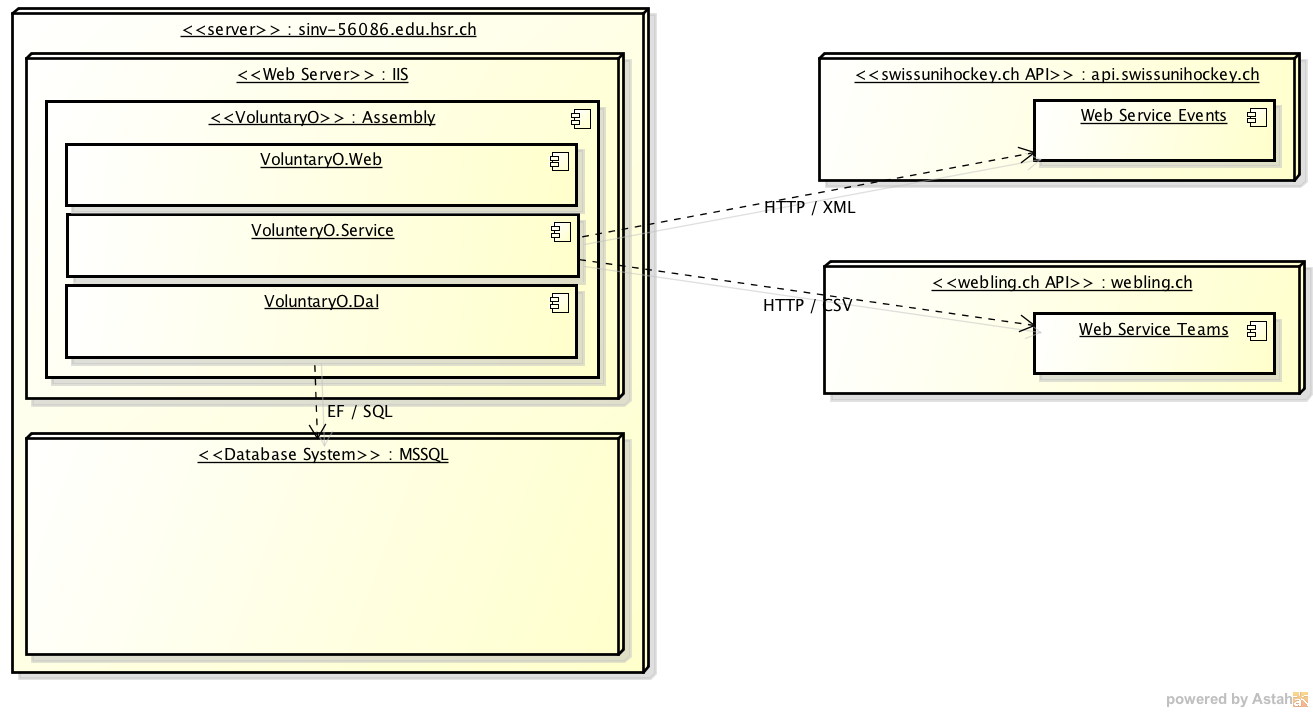
\includegraphics[width=\textwidth]{content/architekturdokumentation/images/deployment.png}

	Das Deployment wird über die Visual Studio Funktion Web Deploy angeboten. Auf dem Server läuft der Dienst für Web Deployment, sodass man aus Visual Studio direkt über den Port 80 den Deploymentdienst aufrufen kann.
	Dann wird ein vorkompiliertes Package direkt aus Visual Studio an den Server übertragen. Die Connection Strings zur Datenbank werden direkt im App.Config geändert, sodass auf dem Server die Connection richtig ist.
	Durch diese Konfiguration lässt sich direkt aus Visual Studio mithilfe eines Klicks die gesamte Applikation auf dem Webserver deployen.
	Vor jedem Deploy sollte alle Unit-Tests ausgeführt werden.
    %!TEX root = ../../architekturdokumentation.tex
\chapter{Datenspeicherung}
    %!TEX root = ../../architekturdokumentation.tex
\chapter{Grössen und Leistung}
Im Rahmen des Projekts sollten rund 250 Benutzer verwaltet werden. Im Verein sind mehrere Mannschaften mit durchschnittlich 15 bis 20 Mitglieder. Zu Spitzenzeiten rechnen wir mit 30 gleichzeitig aktiven Sitzungen (kurz vor Ablauf der Sperrzeit).
Ein durchschnittlicher Event beinhaltet 10 bis 15 freie Helfereinsätze, diese Zahl kann jedoch nach Event- grösse variieren. Pro Woche werden durchschnittlich zwei Events durchgeführt.
Die Datenbank sollte eine Grösse von maximal 50-100 MB nicht übersteigen.

	
    % \chapter{Playground}
\section{A Playground section}        

\subsection{hoi test SUBSUB Section}
\subsubsection{hoi test SUBSUB Section}
Lorem ipsum dolor sit amet, consectetuer adipiscing elit. Aenean commodo ligula eget dolor. Aenean massa. Cum sociis natoque penatibus et magnis dis parturient montes, nascetur ridiculus mus. Donec quam felis, ultricies nec, pellentesque eu, pretium quis, sem. Nulla consequat massa quis enim. Donec pede justo, fringilla vel, aliquet nec, vulputate eget, arcu.

In enim justo, rhoncus ut, imperdiet a, venenatis vitae, justo. Nullam dictum felis eu pede mollis pretium. Integer tincidunt. Cras dapibus. Vivamus elementum semper nisi. Aenean vulputate eleifend tellus. Aenean leo ligula, porttitor eu, consequat vitae, eleifend ac, enim. Aliquam lorem ante, dapibus in, viverra quis, feugiat a, tellus.

Phasellus viverra nulla ut metus varius laoreet. Quisque rutrum. Aenean imperdiet. Etiam ultricies nisi vel augue. Curabitur ullamcorper ultricies nisi. Nam eget dui. Etiam rhoncus. Maecenas tempus, tellus eget condimentum rhoncus, sem quam semper libero, sit amet adipiscing sem neque sed ipsum. Nam quam nunc, blandit vel, luctus pulvinar, hendrerit id, lorem. Maecenas nec odio et ante tincidunt tempus. Donec vitae sapien ut libero venenatis faucibus. Nullam quis ante. Etiam sit amet orci eget eros faucibus tincidunt. Duis leo. Sed fringilla mauris sit amet nibh. Donec sodales sagittis magna. Sed consequat, leo eget bibendum sodales, augue velit cursus nunc,

\section{Code Listings}
\begin{lstlisting}[language=CSharp, caption=Hello World in C\#, label=lst:helloWorldCSharp, firstnumber=1]
// A Hello World! program in C#.
using System;
namespace HelloWorld
{
    class Hello 
    {
        static void Main() 
        {
            Console.WriteLine("Hello World!");

            // Keep the console window open in debug mode.
            Console.WriteLine("Press any key to exit.");
            Console.ReadKey();
        }
    }
}
\end{lstlisting}

\begin{lstlisting}[language=JavaScript, caption=JavaScript Hello Wordl, label=lst:helloWorldJavaScript, firstnumber=1]
//Ausgabe von Hallo Welt! mit einer Alert-Box
alert("Hallo Welt!");
\end{lstlisting}

\section{Text}
Eine ``Beispiel'' Auflistung
\begin{itemize}
    \item Item mit \emph{krusivem} Text
    \item Item mit \textbf{fettem} Text
\end{itemize}

\subsection{Bild}
\begin{figure}[ht]
    
\includegraphics[height=5cm]{template/images/hsrlogo.png}
    \caption{HSR Logo}
\end{figure}


\chapter{Tables}
\section{Meilensteine}

\begin{table}[H]
    \tablestyle
    \tablealtcolored
    \begin{tabularx}{\textwidth}{l l l X}
        \tableheadcolor
            \tablehead ID &
            \tablehead Meilenstein &
            \tablehead Termin &
            \tablehead Beschreibung \tabularnewline
        \tablebody
            \textit{M1}\label{M1} & Ende Inception & 07.03.2014
                & bla bla bla \tabularnewline
            \textit{M2} & Ende Elaboration & 17.03.2014
                & Bla bla bla \tabularnewline
            \textit{..} & .. & ..
                & .. \tabularnewline
            \textit{..} & .. & ..
                & .. \tabularnewline
        \tableend
    \end{tabularx}
    \caption{Meilensteine}
\end{table}

\begin{table}[H]
    \tablestyle
    \tablealtcolored
    \begin{tabularx}{\textwidth}{l X l}
        \tableheadcolor
            \tablehead Topic &
            \tablehead Erläuterung \tabularnewline
        \tablebody
        \textit{Lorem 1} &
            Lorem ipsum dolor sit amet, consectetuer adipiscing elit. Aenean commodo ligula eget dolor. Aenean massa. Cum sociis natoque penatibus et magnis dis parturient montes, nascetur ridiculus mus. Donec quam felis, ultricies nec, pellentesque eu, pretium quis, sem. Nulla consequat massa quis enim. Donec pede justo, fringilla vel, aliquet nec, vulputate eget, arcu.
            \tabularnewline
        \textit{Lorem 2} &
            In enim justo, rhoncus ut, imperdiet a, venenatis vitae, justo. Nullam dictum felis eu pede mollis pretium. Integer tincidunt. Cras dapibus. Vivamus elementum semper nisi. Aenean vulputate eleifend tellus. Aenean leo ligula, porttitor eu, consequat vitae, eleifend ac, enim. Aliquam lorem ante, dapibus in, viverra quis, feugiat a, tellus.
            \tabularnewline
        \textit{Lorem 3} &
            Phasellus viverra nulla ut metus varius laoreet. Quisque rutrum. Aenean imperdiet. Etiam ultricies nisi vel augue. Curabitur ullamcorper ultricies nisi. Nam eget dui. Etiam rhoncus. Maecenas tempus, tellus eget condimentum rhoncus, sem quam semper libero, sit amet adipiscing sem neque sed ipsum. Nam quam nunc, blandit vel, luctus pulvinar, hendrerit id, lorem. Maecenas nec odio et ante tincidunt tempus. Donec vitae sapien ut libero venenatis faucibus. Nullam quis ante. Etiam sit amet orci eget eros faucibus tincidunt. Duis leo. Sed fringilla mauris sit amet nibh. Donec sodales sagittis magna. Sed consequat, leo eget bibendum sodales, augue velit cursus nunc,
            \tabularnewline
        \tableend
    \end{tabularx}
    \caption{Topic Listing}
\end{table}

\begin{table}[H]
    \newcolumntype{s}{>{\centering\hsize=0.15\hsize}X}
    \tablestyle
    \tablealtcolored
    \begin{tabularx}{\textwidth}{X s s s s s s s}
        \tableheadcolor
            \tablehead &
            \rotatebox{90}{\bfseries\textit{TK1 Eigenkonzepte} } &
            \rotatebox{90}{\bfseries\textit{TK2 Eignung}} &
            \rotatebox{90}{\bfseries\textit{TK3 Produktreife}} &
            \rotatebox{90}{\bfseries\textit{TK4 Aktualität}} &
            \rotatebox{90}{\bfseries\textit{TK5 ``Ease of use''}} &
            \rotatebox{90}{\bfseries\textit{TK6 Testbarkeit}} &
            \rotatebox{90}{\bfseries\textit{Gesamtbewertung}}
            \tabularnewline
        \tablebody
            \textit{Ruby on Rails} &
            \oneStar &
            \oneStar &
            \threeStars &
            \oneStar &
            \threeStars &
            \twoStars &
            4
            \tabularnewline
        \tableend
    \end{tabularx}
    \caption{Bewertung Ruby on Rails}
\end{table}

\begin{figure}[H]
    \begin{table}[H]
        \tablestyle
        \tablealtcolored
        \begin{tabularx}{\textwidth}{l c c X}
            \tableheadcolor
                \tablehead Richtlinie &
                \tablehead\rotatebox{90}{Nutzen} &
                \tablehead\rotatebox{90}{Demonstriert\hspace{3mm}} &
                \tablehead Bemerkung
                \tabularnewline
            \tablebody
                Richtline 1 & \faSmile & \faOk & Wiederverwendbare API umgesetzt\tabularnewline
                Richtline 2 & \faSmile & \faOk & Facebook als Identity-Provider\tabularnewline
                Richtline 3 & \faMeh & \faOk & \tabularnewline
                Richtline 4 & \faSmile & \faOk & Make\tabularnewline
            \tableend
        \end{tabularx}
    \end{table}
    \caption{Übersicht Architekturrichtlinienanalyse (2/2)}
    \label{tab:overview-principle-demonstration-2}
\end{figure}

\begin{figure}[H]
    \begin{table}[H]
        \tablestyle
        \tablealtcolored
        \begin{tabularx}{\textwidth}{X | c c c c c | c c c c | c c}
            \tableheadcolor
                \tablehead &
                \multicolumn{5}{c|}{\bfseries\textit{Backend}} &
                \multicolumn{4}{c|}{\bfseries\textit{Frontend}} &
                \bfseries\textit{Tools}
                \tabularnewline
            \tableheadcolor
                \tablehead &
                \rotatebox{90}{Models} &
                \rotatebox{90}{Businesslogik} &
                \rotatebox{90}{Autentifizierung} &
                \rotatebox{90}{Rendering Engine} &
                \rotatebox{90}{Service Interface} &
                \rotatebox{90}{HTML Markup} &
                \rotatebox{90}{CSS Styling} &
                \rotatebox{90}{JavaScript Code} &
                \rotatebox{90}{Struktur} &
                \xspace
                \tabularnewline
            \tablebody
                RP1 REST & & & & & \faOk & & & & & \tabularnewline
                RP2 Application logic & & \faOk & & & & & & & & \tabularnewline
                RP3 HTTP & & & & & \faOk & & & & & \tabularnewline
                RP4 Link & & & & & \faOk & & & & \faOk & \tabularnewline
                RP5 Non-Browser & & & & & \faOk & & & & & \tabularnewline
                RP6 Should-Formats & & & & & \faOk & & & & & \tabularnewline
                RP7 Auth & & & \faOk & & & & & & & \tabularnewline
                RP8 Cookies & & & \faOk & & \faOk & & & & & \tabularnewline
                RP9 Session & & & \faOk & & & & & & \faOk & \tabularnewline
                RP10 Browser-Controls & & & & \faOk & & & & \faOk & \faOk & \tabularnewline
                RP11 POSH & & & & \faOk & & \faOk & \faOk & & & \tabularnewline
                RP12 Accessibility & & & & \faOk & & \faOk & \faOk & & & \tabularnewline
                RP13 Progressive Enhancement & & & & & & \faOk & \faOk & \faOk & & \tabularnewline
                RP14 Unobtrusive JavaScript & & & & & & \faOk & & \faOk & & \tabularnewline
                RP15 No Duplication & \faOk & \faOk & & \faOk & &  \faOk &  \faOk & \faOk & & \tabularnewline
                RP16 Know Structure & & & & & \faOk & \faOk & \faOk & & & \tabularnewline
                RP17 Static Assets & & & & & & & \faOk & \faOk & & \faOk \tabularnewline
                RP18 History API & & & & & & & & \faOk & & \tabularnewline
                TP3 Eat your own API dog food & & & & & \faOk & & & & & \tabularnewline
                TP4 Separate user identity and sign-up (...) & & & \faOk & & & & & & & \tabularnewline
                TP7 Apply the Web instead of working around & & & & & \faOk & \faOk & \faOk & \faOk & \faOk & \tabularnewline
                TP8 Automate everything or you will be hurt & & & & & & & & & & \faOk \tabularnewline
            \tableend
        \end{tabularx}
    \end{table}
    \caption{Mapping Architekturrichtlinien - Systemkomponenten}
    \label{fig:how-to-show-principles-matrix}
\end{figure}


\chapter{New Page}
\newpage
\section{New Paged}

    
    
\end{document}
